%%%%%%%%%%%%%%%%%%%%%%%%%%%%%%%%%%%%%%%%%%%%%%%%%%%%%%%%%%%%%%%%%%%%%
%% This is a (brief) model paper using the achemso class
%% The document class accepts keyval options, which should include
%% the target journal and optionally the manuscript type.
%%%%%%%%%%%%%%%%%%%%%%%%%%%%%%%%%%%%%%%%%%%%%%%%%%%%%%%%%%%%%%%%%%%%%
\documentclass[journal=jpcbfk,manuscript=article]{achemso}

%\documentclass[english,aps,preprint,pre,floatfix,nofootinbib,showpacs,showkeys]{revtex4-1}
%%%%%%%%%%%%%%%%%%%%%%%%%%%%%%%%%%%%%%%%%%%%%%%%%%%%%%%%%%%%%%%%%%%%%
%% Place any additional packages needed here.  Only include packages
%% which are essential, to avoid problems later. Do NOT use any
%% packages which require e-TeX (for example etoolbox): the e-TeX
%% extensions are not currently available on the ACS conversion
%% servers.
%%%%%%%%%%%%%%%%%%%%%%%%%%%%%%%%%%%%%%%%%%%%%%%%%%%%%%%%%%%%%%%%%%%%%
\usepackage[version=3]{mhchem} % Formula subscripts using \ce{}

\SectionNumbersOn

%include hyperlinks to figures
%\documentclass{article}
\usepackage{graphicx}
\usepackage[%  
    colorlinks=false,
    pdfborder={0 0 0},
    linkcolor=blue
]{hyperref}

\usepackage{amsmath}
\usepackage{amssymb}
\usepackage{color}
\usepackage{CJK}
\usepackage{framed}
%\usepackage[hidelinks]{hyperref}
%\usepackage{algorithm}
%\usepackage{algpseudocode}
%\algdef{SE}[DOWHILE]{Do}{doWhile}{\algorithmicdo}[1]{\algorithmicwhile\ #1}

\usepackage[scaled=0.85]{beramono}
\usepackage[T1]{fontenc}
\usepackage{changepage}
\usepackage{mathrsfs}

%%%%%%%%%%%%%%%%%%%%%%%%%%%%%%%%%%%%%%%%%%%%%%%%%%%%%%%%%%%%%%%%%%%%%
%% If issues arise when submitting your manuscript, you may want to
%% un-comment the next line.  This provides information on the
%% version of every file you have used.
%%%%%%%%%%%%%%%%%%%%%%%%%%%%%%%%%%%%%%%%%%%%%%%%%%%%%%%%%%%%%%%%%%%%%
%%\listfiles

%%%%%%%%%%%%%%%%%%%%%%%%%%%%%%%%%%%%%%%%%%%%%%%%%%%%%%%%%%%%%%%%%%%%%
%% Place any additional macros here.  Please use \newcommand* where
%% possible, and avoid layout-changing macros (which are not used
%% when typesetting).
%%%%%%%%%%%%%%%%%%%%%%%%%%%%%%%%%%%%%%%%%%%%%%%%%%%%%%%%%%%%%%%%%%%%%

\makeatletter
    \setlength\@fptop{0\p@}
\makeatother

\newcommand*\mycommand[1]{\texttt{\emph{#1}}}

\newcommand{\state}[1]{$\mathcal{S}_{#1}$}


\newcommand*{\rood}[1]{#1}
\newcommand*{\blauw}[1]{#1}
\newcommand*{\groen}[1]{#1}
\newcommand*{\blauwr}[1]{#1}
\newcommand{\Expect}[1]{\mathrm{E}\left[#1\right]}
\newcommand{\norm}[1]{\left\lVert#1\right\rVert}

%\newcommand*{\addref}[1]{\textcolor{red}{\{ADD REF: #1\}}}

\newcommand*{\noter}[1]{\textcolor{red}{[[#1]]}}		% notes on
%\newcommand*{\noter}[1]{}					% notes off

%\usepackage[draft]{todonotes}   % notes shown
\usepackage[disable]{todonotes} % notes hidden
\usepackage{comment}

\usepackage[normalem]{ulem}
\usepackage{algorithm}
\usepackage{subfig}
\usepackage{algpseudocode}

%%%%%%%%%%%%%%%%%%%%%%%%%%%%%%%%%%%%%%%%%%%%%%%%%%%%%%%%%%%%%%%%%%%%%
%% Meta-data block
%% ---------------
%% Each author should be given as a separate \author command.
%%
%% Corresponding authors should have an e-mail given after the author
%% name as an \email command. Phone and fax numbers can be given
%% using \phone and \fax, respectively; this information is optional.
%%
%% The affiliation of authors is given after the authors; each
%% \affiliation command applies to all preceding authors not already
%% assigned an affiliation.
%%
%% The affiliation takes an option argument for the short name.  This
%% will typically be something like "University of Somewhere".
%%
%% The \altaffiliation macro should be used for new address, etc.
%% On the other hand, \alsoaffiliation is used on a per author basis
%% when authors are associated with multiple institutions.
%%%%%%%%%%%%%%%%%%%%%%%%%%%%%%%%%%%%%%%%%%%%%%%%%%%%%%%%%%%%%%%%%%%%%
\author{Michael S. Jones}
\affiliation{%
  Pritzker School of Molecular Engineering, %
  The University of Chicago, %
  929 East 57th Street, Chicago, Illinois 60637, United States%
}

\author{Brennan Ashwood}
\affiliation{%
  Department of Chemistry, Institute for Biophysical Dynamics, and James Franck Institute, %
  The University of Chicago, %
  929 East 57th Street, Chicago, Illinois 60637, United States%
}

\author{Andrei Tokmakoff}
\affiliation{%
  Department of Chemistry, Institute for Biophysical Dynamics, and James Franck Institute, %
  The University of Chicago, %
  929 East 57th Street, Chicago, Illinois 60637, United States%
}

\author{Andrew L. Ferguson}
\email{andrewferguson@uchicago.edu}
\affiliation{%
  Pritzker School of Molecular Engineering, %
  The University of Chicago, %
  929 East 57th Street, Chicago, Illinois 60637, United States%
}


%\author{Kay T. Finally}
%\affiliation[Unknown University]
%{Department of Chemistry, Unknown University, Unknown Town}
%\alsoaffiliation[Second University]
%{Department of Chemistry, Second University, Nearby Town}

%%%%%%%%%%%%%%%%%%%%%%%%%%%%%%%%%%%%%%%%%%%%%%%%%%%%%%%%%%%%%%%%%%%%%
%% The document title should be given as usual. Some journals require
%% a running title from the author: this should be supplied as an
%% optional argument to \title.
%%%%%%%%%%%%%%%%%%%%%%%%%%%%%%%%%%%%%%%%%%%%%%%%%%%%%%%%%%%%%%%%%%%%%
\title[]{Applying State-free Reversible VAMPNets and Markov State Models to Learn Dynamics of DNA Oligonucleotides}


%%%%%%%%%%%%%%%%%%%%%%%%%%%%%%%%%%%%%%%%%%%%%%%%%%%%%%%%%%%%%%%%%%%%%
%% Some journals require a list of abbreviations or keywords to be
%% supplied. These should be set up here, and will be printed after
%% the title and author information, if needed.
%%%%%%%%%%%%%%%%%%%%%%%%%%%%%%%%%%%%%%%%%%%%%%%%%%%%%%%%%%%%%%%%%%%%%
%\abbreviations{IR -- infrared, NMR -- nuclear magnetic resonance, UV -- ultraviolet}
%\keywords{Takens}

\begin{document}
%%%%%%%%%%%%%%%%%%%%%%%%%%%%%%%%%%%%%%%%%%%%%%%%%%%%%%%%%%%%%%%%%%%%%
%% The manuscript does not need to include \maketitle, which is
%% executed automatically.  The document should begin with an
%% abstract, if appropriate.  If one is given and should not be, the
%% contents will be gobbled.
%%%%%%%%%%%%%%%%%%%%%%%%%%%%%%%%%%%%%%%%%%%%%%%%%%%%%%%%%%%%%%%%%%%%%

\newpage

\begin{abstract}

Despite rapid advances in DNA nanotechnology and a robust understanding of the associated thermodynamics, the sequence-dependent mechanisms of DNA hybridization are not fully understood. In this work, we investigate these dynamics by performing equilibrium coarse-grained simulations of oligonucleotide sequences with varied G:C placement. We employ State-Free Reversible VAMPnets to directly learn the slowest dynamical modes of each sequence and optimize Markov State Model (MSM) construction. Furthermore, we perform elevated temperature simulations to recapitulate temperature-jump IR and FTIR data collected on the oligonucleotides. For repetitive sequences, we find a spectrum of slow dynamics associated with out-of-register base pairing and kinetically relevant transitions between these states. In contrast, G:C pairs near the center of the duplex induce more pronounced fraying dynamics through which hybridization and dissociation are facilitated. In both cases, these mechanisms deviate from an “all-or-nothing” hybridization model. Our computational predictions show agreement with experiments, and provide new fundamental understanding of the sequence-dependent kinetics and mechanisms of DNA hybridization.

% revise "excellent accord" above?

\noindent \url{https://www.overleaf.com/project/5e9e5110c524b8000192c548}

\end{abstract}
%%%%%%%%%%%%%%%%%%%%%%%%%%%%%%%%%%%%%%%%%%%%%%%%%%%%%%%%%%%%%%%%%%%%%
%% Start the main part of the manuscript here.
%%%%%%%%%%%%%%%%%%%%%%%%%%%%%%%%%%%%%%%%%%%%%%%%%%%%%%%%%%%%%%%%%%%%%

\newpage

\section{\label{sec:intro}Introduction}

Over the last couple decades, DNA has proved to be much more than a vessel for genetic information. From sensing, to computing, to directed self-assembly, the programmable and predictable nature of DNA has unlocked numerous unforeseen nanotechnology applications \citep{Seeman2017DNANanotechnology, Adleman1994MolecularProblems, Rothemund2006FoldingPatterns, Gu2010ALine}. In particular, DNA dynamical behavior has become increasingly important in developing these technologies and understanding fundamental biological processes such as transcription and gene regulation \citep{Deluca2020DynamicDevices, Cordes2010SensingTransfer, Naimark2020DNADevelopment}. A thorough understanding of the hybridization process -- the formation of a DNA duplex from two single strands -- and its associated dynamics is integral to further advancements in these fields. The effect of sequence on hybridization thermodynamics has been rigorously explored, and nearest-neighbor calculations can account for mismatched pairs, dangling ends, and other non-native bonding effects \citep{SantaLucia1998AThermodynamics, Santalucia2004TM}. Secondary DNA structures such as hairpins and G-quadruplexes have also been studied in depth and leveraged for nanotechnology applications \citep{Tsukanov2013DetailedOrigami, Mosayebi2014TheFormation, Mergny2019DNANanotechnology}. Although many experimental and computational studies have investigated DNA dynamical phenomena from the picosecond to millisecond range, the sequence-dependent mechanisms of hybridization and dissociation dynamics are not fully understood \citep{Yin2011KineticsHybridization, Xiao2019, Hinckley2014Coarse-grainedEffects, Sanstead2016, Porschke1971CooperativeTransition, Porschke1973ThermodynamicsPairs, Chen2007InfluenceHybridization, Craig1971ElaxationOligon}. Moreover, it is unclear the extent to which these processes evolve in an "all-or-nothing" fashion or if long-lived metastable states facilitate the transition \citep{Araque2016LatticeCooperativity, Sikora2013ModelingIntermediates}.

Our understanding of hybridization dynamics has been built from decades of experiments -- such as temperature-jump, salt-jump, pH-jump, and other perturbative methods -- that rapidly perturb DNA and monitor relaxation to a new equilibrium \citep{Morrison1993SensitiveSolution, Wetmur1968KineticsDNA, Craig1971ElaxationOligon, Porschke1973ThermodynamicsPairs, Williams1989LaserDGCATGC, Narayanan2012ExploringMixing, Chen2007InfluenceHybridization, Sanstead2018DirectDehybridization}. More recently, single molecule diffusion and tethered multifluorophore assays have facilitated equilibrium analysis, however these results can be hampered by slow data collection rates and fluorescent tags effects on strand dynamics, particularly for shorter oligomers \citep{Liu20173DSolution,  Schickinger2018TetheredHelices, Chen2008Base-by-baseSpectroscopy, Dupuis2013Single-moleculeHelices, Morrison1993SensitiveSolution}. Given that dynamic insights from these experiments are limited, several coarse-grained molecular dynamics (MD) models have been employed to provide molecular level detail \citep{Romano2013DNADependence, Hinckley2013AnHybridization, Maciejczyk2014DNAModel, Markegard2015, Dans2016MultiscaleDNA}. Although these models provide experimentally verified speed-ups compared to all-atom simulations, the long timescales on which DNA hybridization and dissociation events occur can still make these processes difficult to sample via direct simulation techniques \citep{Phys2014}. Instead, many previous studies of DNA hybridization have employed accelerated sampling methods such as metadynamics, umbrella sampling,  transition path sampling, and forward flux sampling \citep{Schmitt2013ExploringSurface, Sambriski2009,  Hoefert2011MolecularOligonucleotides, Romano2013DNADependence}. Simplified lattice models can expedite computation time and yield useful thermodynamics and transition state information, however some configurations may not be accessible and kinetics are less informative \citep{Araque2016LatticeCooperativity, Phys2019}. Other computational works use elevated temperature or denaturing solvent concentrations to induce one-way dissociation events \citep{Wong2008TheSimulations, Perez2010Real-timeUnfolding}. Taken together, most experimental and computational work have studied the hybridization process as a relaxation to a chosen equilibrium or in a biased fashion.

Recent studies have coupled experimental techniques with machine learning (ML) and  MD simulations to investigate and predict sequence-dependent kinetics \citep{Schickinger2018TetheredHelices, Zhang2018PredictingSequence}. Where these studies focus on association and dissociation kinetics alone, we seek to broaden our analysis into higher order dynamical processes and metastable intermediates. For example, stable out-of-register or "shifted" base pairing in repetitive sequences have been documented in previous computational studies \citep{Phys2014, Maciejczyk2014DNAModel, Araque2016LatticeCooperativity, Xiao2019}. The extent to which these states are kinetically relevant is difficult to determine experimentally, and appears highly sequence-dependent. Frayed structures and dynamics have also been investigated in numerous computational and experimental studies \citep{Zgarbova2014BaseRNA, Nonin1995TerminalFraying, Nikolova2012ProbingSimulations, Andreatta2006UltrafastHelix}. Sanstead et al. highlighted the role of these dynamics during duplex dissociation, where the stability and relaxation timescale of frayed states was dictated by G:C base placement 10-mer oligonucleotides \citep{Sanstead2016}. Together, these dynamics represent substantial deviations from all-or-nothing behavior that can be variably expressed via subtle sequence differences in short oligomers.

In this work, we study the same four sequences explored by Sanstead et al. in an effort to uncover sequence-dependent dynamics and their relation to metastable structures mentioned above \citep{Sanstead2016}. We use the coarse-grained 3 Sites per Nucleotide (3spn2) model to perform unbiased simulations of hybridization and dissociation behavior near each sequence's melting temperature \citep{Hinckley2013AnHybridization}. We synthesize the simulation trajectories using Markov State Models (MSMs) to combine many independent and unbiased trajectories and develop an understanding of sequence-specific kinetics and thermodynamics \citep{Pande2010EverythingAsk}. MSMs have recently been implemented to study mechanisms and microstate distributions of DNA hybridization, but the slowest sequence-dependent kinetics were not the focus of these studies \citep{Jin2019, Xiao2019}. \citet{Pinamonti2017} used MSMs to compare the slowest dynamics of short RNA nucleotides and found that stacking timescales are highly sequence dependent. We take a similar approach to study 10-mer DNA oligonucleotides and implement state free-reversible VAMPnets (SRVs) within the MSM parameterization pipeline to construct higher resolution kinetic models than are achievable using standard time-lagged independent components analysis (tICA) based approaches.

% this section should look more like a conclusion foreshadowing conclusions and main take aways 
We find that 3spn2 allows us to access long length and time scales and observe sequence-dependent kinetics and relaxation rates that are, within a corrective scaling factor, in agreement with observed experimental trends. Applying SRV-MSMs enables the construction of high-resolution sequence-dependent kinetic models of hybridization and dissociation. Consistent with previous studies \citep{Phys2014,Romano2013DNADependence,Araque2016LatticeCooperativity}, we find the degree of repetitiveness in the sequence and therefore the kinetic accessibility and thermodynamic stability of shifted states leads to richer folding dynamics populated by a diversity of long-lived metastable states. Disrupting repetitive stretches of bases by judicious placement of interrupting G:C pairs can tune the landscape from rich 6-state to very simple 2-state (“all-or-nothing”) behavior. Furthermore, concentrating G:C pairs at the center of a duplex produces a longer-live frayed state that facilitates the hybridization and dissociation process. Analysis within metastable state populations using diffusion maps allows us to explore the conformational diversity and heterogeneity within each state at time scales shorter than the kinetic resolution of the SRV-MSMs. This provides us with molecular-level understanding for the differential stability of various conformational states as a function of oligomer sequence. Taken together, our analysis reflects similar results to previous computational and experimental DNA work, while elucidating new insights into sequence-dependent dynamics, metastable structures, and relative timescales. 

% example text from Andy's conclusions:

% Correlation of the data-driven kinetic order parameters extracted by SRVs provides new understanding of the sequence-dependent kinetic mechanisms by which oligomers hybridize and reveal these to be richer than classical base-pair shifting and “all-or-nothing” behaviors.

% original last paragraph
%By evaluating equilibrium trajectories we can study the relevance of metastable states during both the hybridization and dissociation process. Because SRVs generate an optimized low dimensional basis, we show that higher resolution MSMs (measured by a reduction in the required lag time) are accessible. Additionally, we compare slow dynamical modes and metastable states between sequence-specific SRV-MSMs. Within these metastable dynamical states, we leverage diffusion maps to analyze the diversity of structures whose inter-conversion rate are too fast to produce unique slow modes. Finally, we run higher temperatures simulations to investigate the temperature-dependent nature of some experimentally relevant dynamical responses. Taken together, our analysis reflects similar results to previous computational and experimental DNA work, while elucidating new insights into sequence-dependent dynamics, metastable structures, and relative timescales. 


%These studies have fueled increasingly complex structural DNA technologies, but developments in dynamic DNA nanotechnologies have outpaced our understanding of the dynamics themselves \citep{Deluca2020DynamicDevices}. 

%Still, rich dynamics have been observed short nucleotides \citep{Sanstead2018DirectDehybridization} and the sequence-dependent effects on these dynamics are not well understood.

%Progress has also been made in modeling kinetics for certain dynamic DNA systems, such as toehold exchanges and optical barcodes \citep{Zhang2009ControlExchange, Shah2019ProgrammingFingerprinting}. Sequence effects on association and dissociation rates were predicted using combined experimental and machine learning approaches, however higher order dynamics are less well understood \citep{Zhang2018PredictingSequence}.  Hairpin \citep{Woodside2006DirectAcid} and in duplex hybridization \citep{yer2014KineticsAT-tracts, Sanstead2016, Sanstead2018DirectDehybridization} studies have revealed sequence-dependent effects and varied differential deviations from "all or nothing" behavior. In temperature-jump spectroscopy, G:C placement alters the slow kinetic response attributed to dissociation and a fast response likely corresponding to terminal A:T fraying. Experimentally, however, it is difficult to pick up on dynamics that have similar spectroscopic signatures and to tease apart temporally close responses that might be combined into one stretched exponential signal. 

% include Tokmakoff conclusions in the intro -- sequence-dependent deviations from two-state behavior. The slow response was attributed to complete strand dissociation, while the fast response described base fraying. We perform longer equilibrium sampling near Tm to get a sense of sequence equilibrium behavior, as well shorter simulations at a range of higher temperatures to replicate T-jump data. Taken together, our analysis reflects similar results to previous computational and experimental DNA work, while elucidating new insights into sequence-dependent dynamics, metastable structures, and relative timescales. 

\section{\label{sec:methods}Methods}

\subsection{\label{sec:methods}Simulation set up}

The 3 site per nucleotide (3spn2) coarse grained model was designed to accelerate DNA computation relative to all-atom models while maintaining experimental melting temperatures, stacking energies, and persistence lengths\citep{Hinckley2013AnHybridization}. Interaction sites are located at phosphate, sugar, and base centers of mass; anisotropic potentials are designed to model non-bonded interactions such as intra-strand base-stacking, inter-strand cross-stacking, and base pairing. The model has been validated against experimentally determined structural properties and hybridization rates, although no dynamic information was used to parameterize the model other than Langevin friction coefficients \citep{Hinckley2013AnHybridization, Hinckley2014Coarse-grainedEffects}. The 3spn2 model been has widely-adopted to study numerous phenomenon including DNA packing in viral capsids, protein-DNA binding, and nucleosome unwrapping. \citep{Cordoba2017AIons, Lu2020OpenAWSEMSummary, Lequieu2016Tension-dependentUnwrapping}. 

We initialized four self-complementary double-stranded sequences previously the subject of ultra-fast T-jump experimentation -- 5'ATATATATAT3' (AT-all), 5'GATATATATC3' (GC-end), 5'ATATGCATAT3' (GC-core), and 5'ATGATATCAT3' (GC-mix) -- in a periodic box of dimensions 7.8 nm \citep{Sanstead2016, Phys2014}. We specified a 240 mM implicit salt concentration and used a Debye-Huckel approximation for electrostatic interactions within a 5 nm cutoff. We ran our simulations in the NVT ensemble. Temperature was controlled by a Langevin thermostat that models interactions with an implicit water solvent. \citep{Schneider1978Molecular-dynamicsTransitions}. Simulations were conducted at empirically determined  melting temperatures in order to observe frequent transitions between dissociated and hybridized states. We used a 20 fs time step and $1.3\times10^{9}$ steps in each simulation, saving frames every 100 ps. For each sequence, 40 simulations were performed in parallel, consuming about 24 serial CPU-hours on 28xIntel E5-2680v4 processors per simulation. Half of runs were initialized from the native hybridized state and half from a dissociated state. The first 10000 frames (1 $\mu$s of simulation time) of each simulation were removed, resulting in 40 x 250000 frames and a total of 1 ms simulation time per sequence. We observed between 55-100 hybridization/dissociation events for each of the four sequences.

\subsection{\label{sec:methods}Featurization}

A featurization of trajectories was required to capture fundamental dynamics while accounting for translational and rotational symmetries. Pairwise distances between base centers of mass -- similar to heavy atom distances in protein models \citep{Sidky}-- satisfied these requirements and were calculated at each frame using the MDtraj Python library \citep{McGibbon2015MDTraj:Trajectories}. Although pairwise distances remove translational and rotational symmetries, additional symmetries arise from the self-complementary nature of these sequences -- the sense and anti-sense strands in each pair are identical to each other. To account for this, we averaged permutable distances (45 pairs in total) together into a "symmetrized" feature set following a similar procedure used in tICAgg coordinates construction \citep{Sengupta2019AutomatedSelf-assembly}. The VAMP-2 scoring method was employed to evaluate the kinetic variance of the feature set and optimize hyperparameters \citep{WuVariationalData, Mardt2018VAMPnetsKinetics}. Additional details on the VAMP-2 score can be found in the supplemental information. By comparing scores across several candidate feature sets (figure \ref{fig:allseq_features_vamp2}), we found that minimal kinetic information was lost in the  symmetrization procedure. Furthermore, the smaller feature set enabled faster training times and better statistics over permutable distances, without appearing to suffer a loss in generality or model resolution.  

\begin{figure}[ht!]
	\begin{center}
        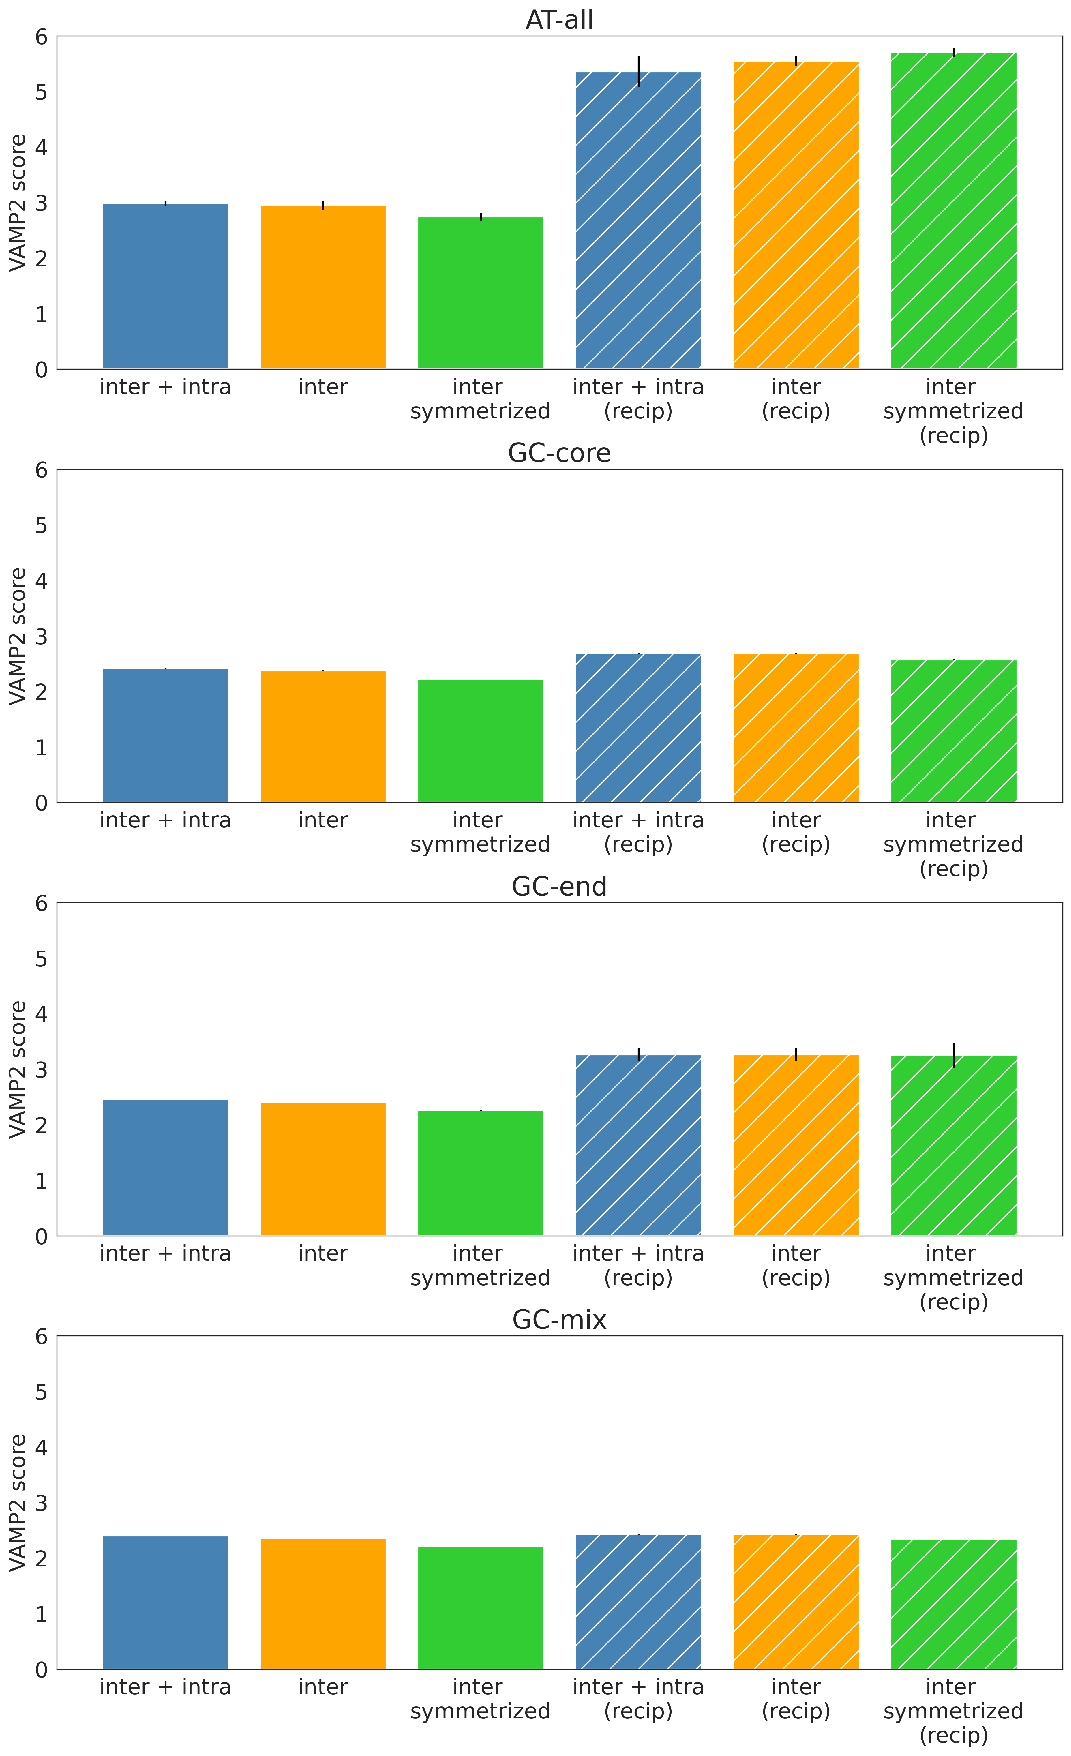
\includegraphics[width=80mm,
        scale=0.5]{Fig1.pdf}
        \caption{A comparison of VAMP-2 scores via 5-fold cross-validation for the intermolecular, intra+intermolecular,  and symmetrized intermolecular distances, in addition to the reciprocal value for each of these coordinates. Reciprocal coordinates performed better across the board, but there was no substantial difference between the three featurization methods. This indicated that minimal kinetic information was lost in the symmetrization procedure, therefore we chose reciprocal symmetrized coordinates to train the model.}
        \label{fig:allseq_features_vamp2}
	\end{center}
\end{figure}


\subsection{\label{sec:methods}SRVs}
 
The next step in the MSM pipeline is to create a low-dimensional kinetic projection where state clustering is performed. While most pipelines employ tICA to generate a linear transformation of input features, we use SRVS as a more powerful modular replacement for tICA. SRVs were first developed by Chen et al. as a means to directly learn slow eigenfunctions of the transfer operator \citep{Chen}. The method is a descendant of VAMPnets \citep{Mardt2018VAMPnetsKinetics}, deep canonical correlation analysis \citep{Andrew2013DeepAnalysis}, and extended dynamic mode decomposition with dictionary learning (EDMD-DL) \citep{Li2017ExtendedOperator}. The framework uses a twin-lobed artificial neural network to learn an optimal basis set for the variational approach to conformational dynamics (VAC) from which the leading eigenfunctions of the transfer operator are then estimated \citep{Noe2013ASystems}. The resulting orthogonal modes are associated with the slowest dynamical processes in a system, and can be used to interpret kinetic information directly (such as physical correlations and timescales) and to construct MSMs \citep{Sidky, Pande2010EverythingAsk}. SRVs provide robust nonlinear approximation and computation time that scales linearly with the amount of input data and are more powerful and efficient that tICA and ktICA approaches. This is a key attribute to our system as 10 million frames with 55 features in each frame are used for each sequence. The SRV framework has been used to construct high kinetic resolution MSMs applied to molecular simulations of WW-domain and Trp-cage mini-protein \citep{Chen, Sidky}. 

\subsection{\label{sec:methods}SRV-MSMs}

% need some more detail here -- talk to Andy about this
MSMs are a powerful tool for interpreting large amounts of simulation data in a statistically robust and experimentally comparable way \citep{Phys2011MarkovValidation, Husic2018MarkovScience}. After Kinetically similar conformations are first discretized into microstates and the conditional probability of transition between state is calculated within some lag time. The reliance on conditional probabilities allows for many independent simulations (longer than the lag time) to be collectively interpreted. To take full advantage of the MSM frameworks, however, the input basis should be as kinetically meaningful as possible \citep{Pande2010EverythingAsk}. Because SRV eigenfunctions translate simulation features into their slowest kinetic representations, they are optimally suited as an MSM basis. To build our SRV-MSM framework, we employed the PyEmma MSM pipeline and generated independent models for each sequence \citep{Scherer2015PyEMMAModels}. In a similar approach to Sidky et al. we performed k-means microstate clustering, Bayesian MSM construction, and PCCA+ hierarchical macrostate assignments \citep{Sidky}. The number of microstates were determined by VAMP-2 score, and the SRV-MSM lag time was selected based on implied timescales convergence.  The number of PCCA+ macrostates was determined based on the characteristic of each system and will be discussed more in depth in the results and supplemental information.

%%%%%%%% Methods comments %%%%%%%%%%%%%%%%%

%We found close agreement with explicit ion simulations performed with 240 mM \ce{NaCl} and 18 mM \ce{MgCl2} (supplemental) but 7x slower simulation speed made adequate sampling more difficult to achieve under these conditions.

%We initialized explicit ions such that 240 mM \ce{NaCl} and 18 mM \ce{MgCl2} were added to the box in addition to 18 Na counter ions to balance the charge from the 9 phosphate groups in each oligonucleotide backbone \citep{Hinckley2015}. We used a periodic box size of 7.774 nm and an effective oligo concentration of 7 mM. We used an Ewald summation to calculate long range Coulombic interaction between DNA and ions using a real space cutoff of 2 nm.

%%%%%%%%%%%%%%%%%%%%%%%%%%%%%%%%%%%%%%%%%%%%%%%%%%%%%%%%%%%%%%%%


\section{\label{sec:Results}Results}

% Include analysis on overall hybridization rates here or at the end?

\subsection{Sequence-dependent coarse-grained kinetics agree with T-jump IR data}

% rerun these at the actual final temps and just see what happens? Doesn't really matter where Tjump occurs and could make things easier as a whole...
% talk about rerunning AT-all and GC-mix=

As an initial validation of the 3spn2 kinetics, we compared simulated relaxation measurements with temperature-jump (T-jump) experiments. Coarse-grained timescales are inherently difficult to match against experiments due to smoothing of the free energy landscape and variable acceleration across different degrees of freedom. As such, we evaluated multiple temperatures for each sequence and inferred acceleration factors from temperature-dependent trends.  Experimental temperature-dependent relaxation timescales were measured for each sequence using T-jump IR spectroscopy as described previously \citep{Sanstead2018DirectDehybridization}. We recorded "fast" and "slow" amplitude-weighted responses -- previously attributed to terminal base pair fraying and duplex dissociation, respectively -- for each temperature and sequence. To compare results with 3spn2, we ran 120 shorter (1 us) simulations initialized in the hybridized state at final T-jump temperatures for each sequence. We derived relaxation times for a slow dissociation response and fast fraying response at each temperature and compared these with experimental temperature-dependent relaxation fits.

% need to discuss tmelt shift
We measured the slow dissociation response by fitting the distribution of times at which the core base pairs separate beyond a 2 nm cutoff. We found the inverse of these relaxation times -- the effective dissociation rate -- to increase exponentially with temperature, which is expected given the large enthalpic barrier of dissociation \citep{Craig1971ElaxationOligon,Porschke1971CooperativeTransition,Williams1989LaserDGCATGC}. We noted an average temperature shift of about 4C between experiment and simulation exponentials. While 3spn2 captures melting temperature relatively well, some deviation is expected given varied ion conditions and other coarse-grained effects. We used to this temperature shift to inform our equilibrium simulations in the proceeding section. We also noted an acceleration of about one order of magnitude compared to experiment, although this factor is sensitive to the exact definition of melting temperature. After accounting for the melting temperature shift and acceleration factor, we saw strong agreement between the experimental data and simulated relaxation fits. At lower temperatures, T-jump slow responses likely contain a mix of dissociation and hybridization dynamics, therefore rates do not drop off to the same extent as our analysis which considers dissociation alone. GC-core showed the largest deviation from experiment, indicating that increased temperature triggers dissociation at a disproportionately higher rate in simulation compared to experiment. 

% GC-core fast timescales could be slower as they have contributions from internal fraying which would have a longer relaxation than the termini alone.
% in order to make comparisons across these different free energy landscapes, we adjusted simulations by a consistent acceleration factor. We maintained a consistent accegqrelation factor across sequences, but found that optical scaling different by about one order of magnitude between fast and slow responses. It is expected given that different degrees of freedom often experience differing amounts of accelerations in coarse-grained models.

% need to update this fig with labels and temp shift

\begin{figure}  %[ht!]
	\begin{center}
        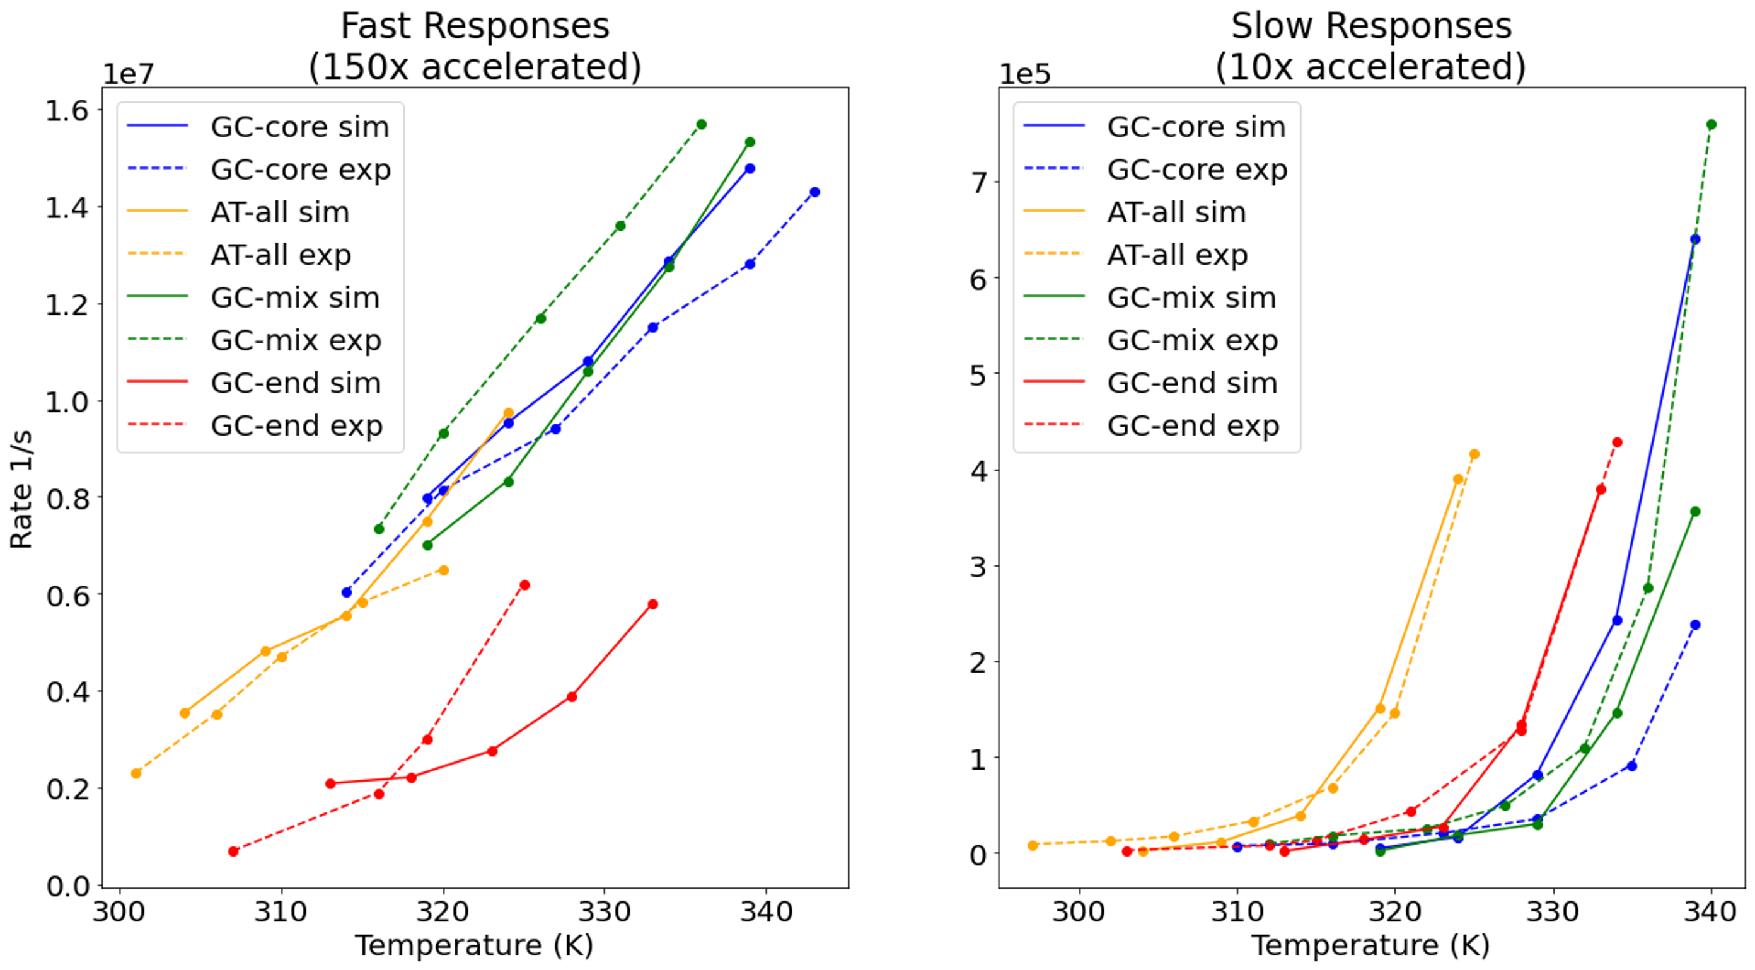
\includegraphics[width=\textwidth]{Fig2.pdf}
        \caption{Fitting temperature-dependent trends to the "slow" dissociation mode and "fast" fraying mode detected in experiments. The effective simulation temperature is shifted by 4 degrees celcius to account for systematic differences in simulation and experimental melting temperature. Different scaling factors are applied to fast and response to account for variable coarse-grained acceleration along different degrees of freedom.}
        \label{fig:relaxation-comparison}
	\end{center}
\end{figure}

% A documented short-coming for the 3spn2 model is a high proclivity for termini fraying relative to what has been observed in vitro \citep{2013}. This supports why we observe significantly more acceleration for the fast response, but relative sequence and temperature effects still compare well with T-jump results.

The fast response -- which Sanstead et. al attributed to terminal base pair fraying signatures -- was more challenging to compare against simulation observables. Numerous experimental and computational studies have shown that DNA and RNA fraying is a complex dynamical process with timescales that span 5 ps to several microseconds \citep{ Nonin1995TerminalFraying, Nikolova2012ProbingSimulations, Andreatta2006UltrafastHelix, Galindo-Murillo2015ConvergenceDGCACGAACGAACGAACGC}. All-atom simulations suggest that frayed ends can assume misaligned WC bonds, base-sugar hydrogen bonds, and terminal stacked conformations \citep{PinamontiTheModels, Zgarbova2014BaseRNA}. Given that there is only one interaction site parameterized on each 3spn2 base, we would not expect to resolve this diverse collection of states and dynamics. Instead, we measured the fast fraying response by counting frames until duplex terminal ends splits beyond a cutoff. This approach assumes that fraying on the permutable top and bottom of the duplex are independent from each other, and that a base pair distance is a reliable approximation for the ensemble spectroscopy signal. This is a reasonable assumption given that the amplitude-weighted timescales should consist largely of terminal fraying events. Again we fit relaxation curves to the ensemble of fraying timescales in order to extract rate approximations for each sequence at a series of temperatures. 

For A:T terminal sequences, the simulated fast response appears linear with temperature, indicating a barrierless and diffusion-driven process. In contrast, the GC-end responses are distinctly slower and increase exponentially with temperature, likely due to a greater enthalpic barrier associated with G:C fraying. We observe similar trends in the experimental data, although comparisons at high temperatures were limited due to mixing between the fast and slow responses (figure \ref{fig:relaxation-comparison}). We found the optimal acceleration factor to be dependent on the choice of the cutoff parameter, but we can approximate that 3spn2 fraying dynamics are accelerated by about 100-200x relative to experiments. It is not surprising that we see different rates of acceleration for the dissociation and fraying processes given that coarse-grained effects can vary across different degrees of freedom. In particular, the simplified treatment of the fraying process may smoothen the free energy landscape and speed up dynamics relative to a more global processes like dissociation. Although one should rely on higher resolution models to study in depth mechanisms of fraying, our results indicate that terminal fraying is a reasonable assignment for the spectroscopic fast response in Sanstead et al. and that 3spn2 can capture some sequence-dependent fraying effects.
% need a better transition here back into SRV-MSMs?

\subsection{SRV-MSMs for each sequence}

% change state names and scientific notation
% include D here? can see what it would look like...
\begin{figure}[ht!]
	\begin{center}
        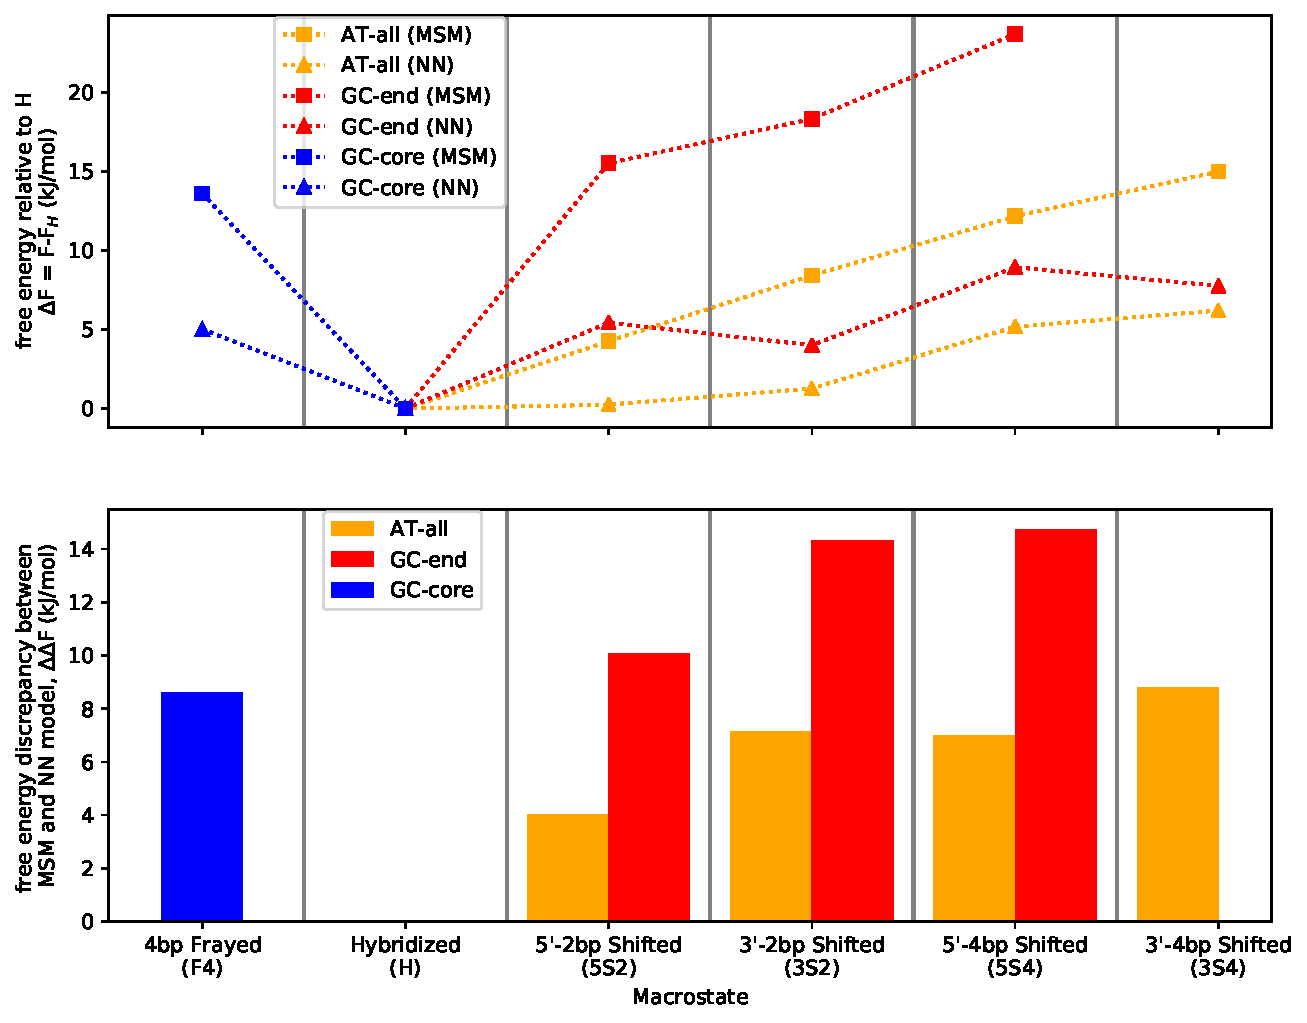
\includegraphics[width=160mm, 
        scale=1]{Fig3.pdf}
        \caption{Nearest neighbor representations, molecular renderings, and sequence-dependent probabilities for PCCA+ macrostates. Shifted state abbreviations indicate the direction of the shifted overhang (5' vs. 3') and the number of shifted motifs relative the native state (1 vs. 2).}
        \label{fig:allseq_table}
	\end{center}
\end{figure}

% potentially get rid of State representation, ask Brennan if they are meaningful?
\begin{figure}[ht!]
	\begin{center}
        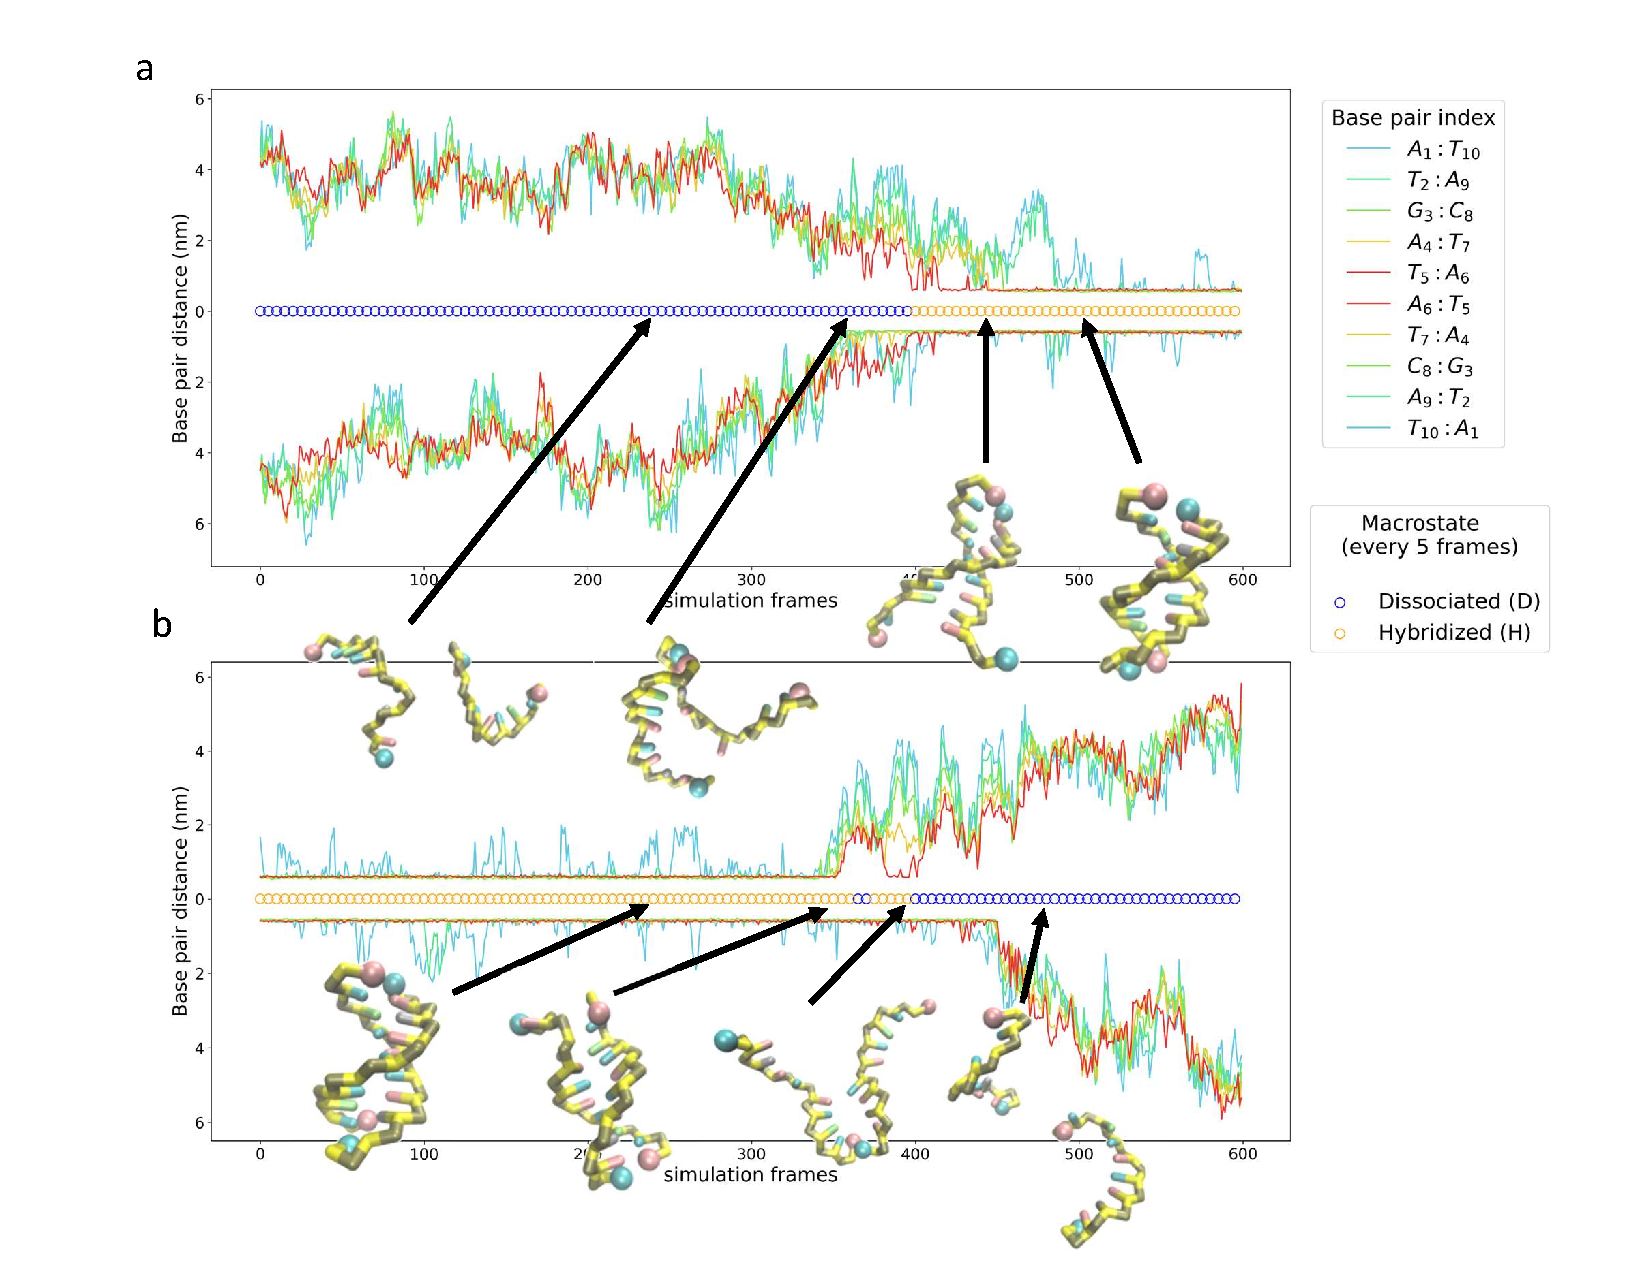
\includegraphics[width=120mm, 
        scale=1]{Fig4.pdf}
        \caption{Flux diagram between PCCA+ states are shown for each sequences, accompanied by representative structures are for each macrostate. Arrows indicate the probability of transitioning out of the state within the lag time. Circle areas are proportional to state stability.}
        
        %Free energies maps and PCCA+ states clusterings are shown in the tICA space in order to enhance visibility in dimensions. }
        \label{fig:allseq_transition}
	\end{center}
\end{figure}

Following the analysis pipeline described above, we generate SRV-MSMs for each sequence. We identified seven kinetically relevant states that are captured within the resolution of the model. Figure \ref{fig:allseq_table} shows cartoon and molecular rendering for each of these states as well as their sequence-specific stationary probabilities. By row, these include the fully hybridized state (H) in which all native base pairings are intact, four "shifted" states (5S1, 3S1, 5S2, 3S2) where complementary base pairs form out-of-register, a frayed state (F4), unique to GC-core, in which the four terminal A:T base pairs are unbound, and the fully dissociated state (D). Figure \ref{fig:allseq_transition} shows how these states fit into sequence-specific low-dimensional representations and kinetic models. Arrows between states show the conditional transition probability to another state within the MSM lag time. We now proceed to analyse the sequence-dependent thermodynamics and kinetic features of each MSM.

%Shifted states are only observed for AT-all and GC-end; state abbreviations indicate the direction of the shifted overhang (5' vs. 3') and the number of shifted motifs relative the native state (1 vs. 2). GC-mix displays two-state behavior within the resolution of the model, however we will show that the hybridization and dissociation are still characterized by an ensemble of shorter-lived states. Stationary probabilities in each of these states are shown in figure \ref{fig:allseq_table}. We also show that PCCA+ clustering assigns states to relative free energy minima in the tICA space.

% rewrite this into one paragraph
\subsection{MSM stabilities agree with nearest neighbor thermodynamic models}

%The repetitive AT motifs in the AT-all and GC-end sequences produces a collection of out-of-register states similar to those shown in previous coarse-grained and all-atom studies \citep{Phys2014,  Romano2013DNADependence, Araque2016LatticeCooperativity, Xiao2019}. The thermodynamic stability of these states can be evaluated against experimental prediction by defining each structure in terms of "dangling ends" -- unpaired bases adjacent to the paired duplex -- and "inert tails" -- free bases that extend beyond the dangling end \citep{Michele2014EHybridization}. Dangling ends tend to have small stabilizing effects, and inert tails decrease stability as they increase in length -- 3' inert tails have stronger effects than 5' tails. Although sequence-dependent effects of inert tails are less well known, dangling end effects can be factored into nearest neighbor (NN) calculations \citep{Santalucia2004TM}. 

Nearest neighbor (NN) models have been experimentally optimized to account for stacking contributions of native pairs, internal mismatches, and dangling ends\citep{Santalucia2004TM}. The effects of inert tails -- free bases that extend beyond the dangling end -- have been shown to destabilize the duplex but are not included in NN models \citep{Michele2014EHybridization}. It is informative to compare our MSM predictions against NN calculations to understand how inert tail and kinetic effects may cause deviation from these predictions. In particular, we examine  the out-of-register AT-all and GC-end states which are amenable to NN comparisons (figure \ref{fig:NN_table}). For AT-all, NN calculations  predict that conformations in the 5' shifted states (5S1 and 5S2) are more energetically favorable than those in the 3' shifted state (3S1 and 3S2). We find qualitative agreement to our macrostate free energies, where inert tail effects likely contribute a 4-6.5 kJ/mol increase in free energy compared to dangling end predictions alone. For GC-end, we consider C:T and G:A mismatches as non-interacting dangling ends such that each shifted conformation has four total dangling ends. Based on this treatment, NN calculations yield higher overall free energies due to fewer native base pair contacts.  Contrary to macrostate results, however, the 3S1 state is more stable than 5S1 states. Moreover, we do not observe a stable 3S2 cluster for GC-end. This indicates that 5' vs. 3' inert tail differences -- attributed to some combination of 5' tails preferentially stacking on the core duplex and 3' tails perturbing the duplex structure -- may out-weight NN stacking effects alone \citep{Doktycz1990ThermodynamicATGC}. 

% and inert tails tend to decrease stability as they increase in length, particularly at lower ionic strengths. It has been shown that 5' dangling ends with one inert tail have higher melting temperatures and are energetically favorable compared to 3' ends \citep{Senior1988InfluenceDuplexes, Dickman2012ThermodynamicDNAs}. These effects might be attributed to some combination of 5' tails preferentially stacking on the core duplex and 3' tails perturbing the duplex structure \citep{Doktycz1990ThermodynamicATGC}. 

% Although NN calculations predict 5' vs. 3' stabilities for AT-all, we observe that GC-end 5S1 state remains more populated than the 3S1 state contrary to NN predictions. Indeed, we do not observe the formation of a stable 3S2 state for GC-end, further indicating that these states 3' states are unfavorable. This leads us to believe that 5' vs. 3' differences -- attributed to some combination of 5' tails preferentially stacking on the core duplex and 3' tails perturbing the duplex structure -- may out-weight NN effects \citep{Doktycz1990ThermodynamicATGC}. 

\begin{figure}[ht!] % right place for NN table? could go to SI
	\begin{center} 
        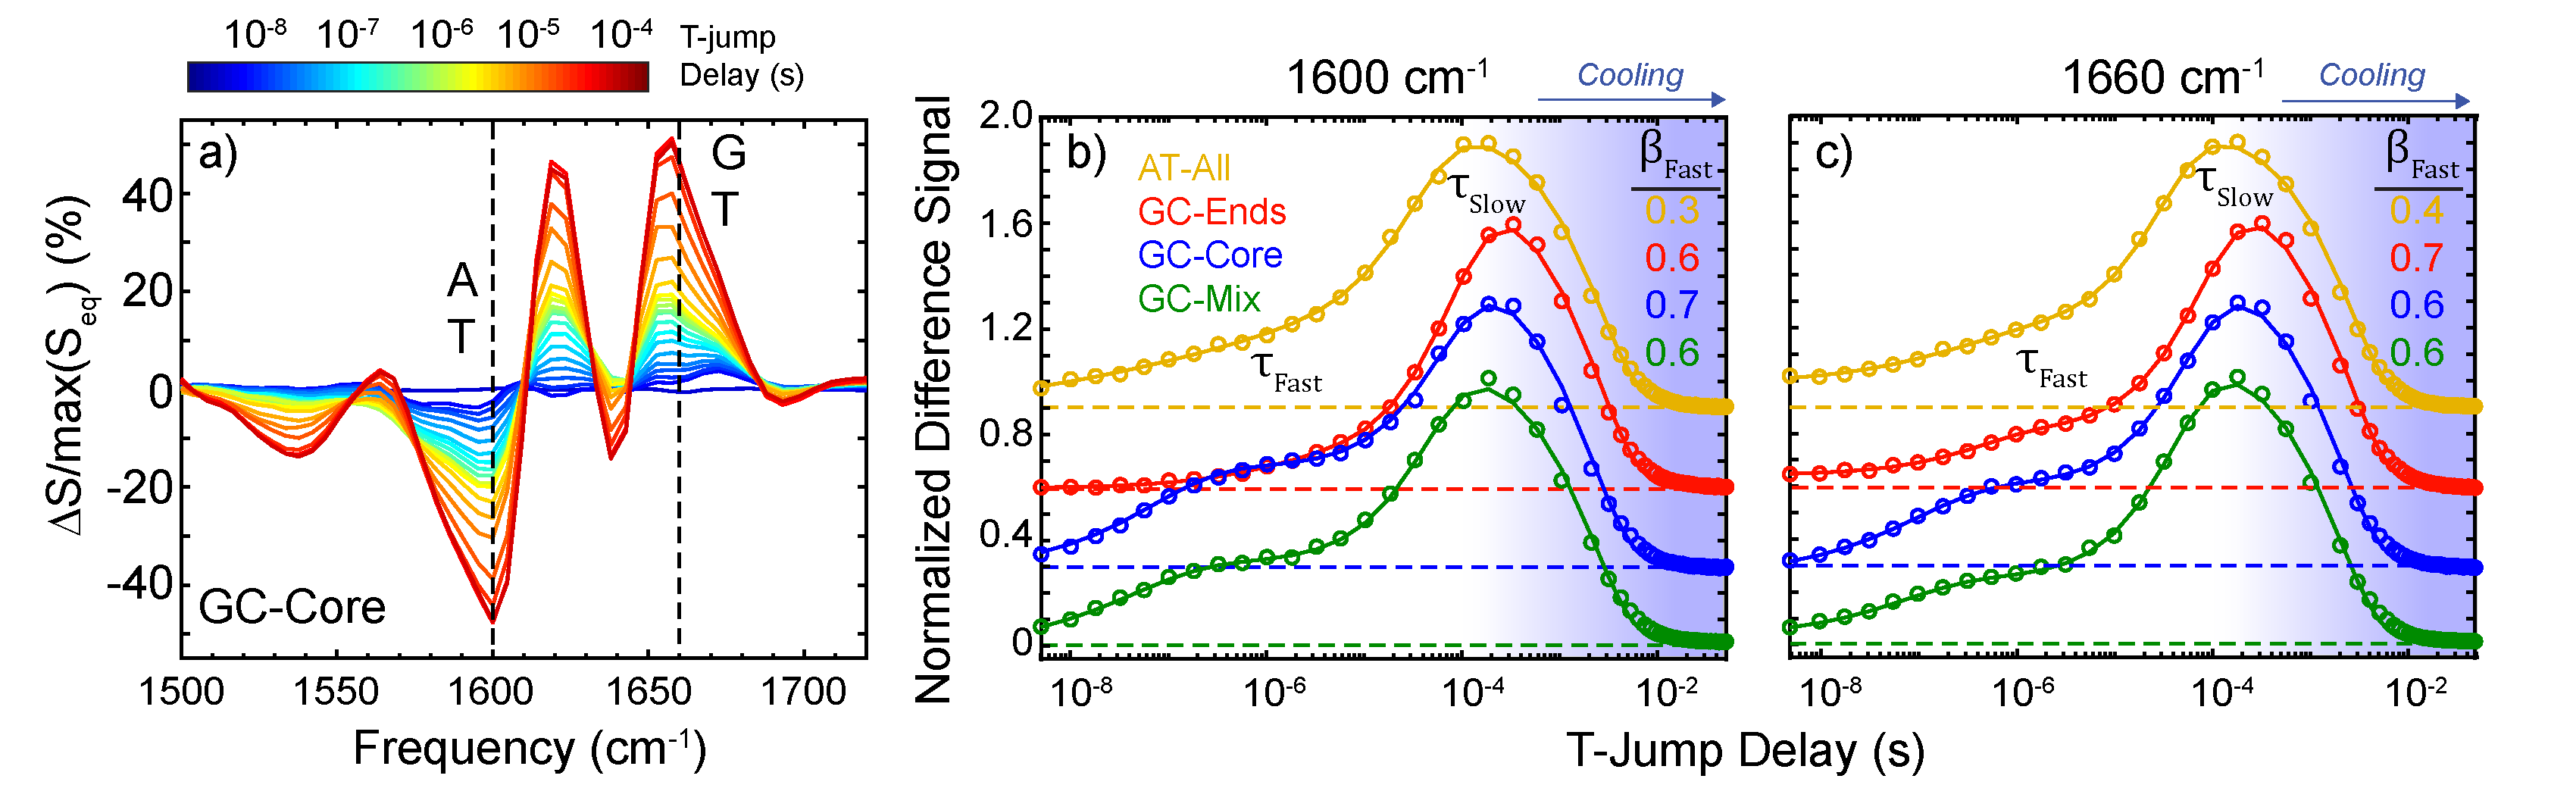
\includegraphics[width=120mm, scale=1]{Fig5.pdf}
        \caption{Comparisons between free energies based on simulation macrostate populations and nearest neighbor calculations. All free energies are normalized such that that the native hybridized state is set to zero. Calculations included dangling end contributions but do not take inert tails effects.}

        \label{fig:NN_table}
	\end{center}
\end{figure}

%if AT-all has highest frequency and GC-end has lowest then can describe role of metastable states as increasing rate for the former but decreasing rate for the later (for kinetic traps that do not terminate in native hybridization and delay the process as a whole).

\subsection{Out-of-register dynamics facilitate hybridization and dissociation}
%\subsubsection{Transition probabilities between states}

In addition to state probabilities and free energy approximations, the coarse-grained MSM yields valuable discrete kinetic information in the form of transition probabilities between states. For AT-all, we observe approximately equal probability of transitioning from D to any other state. Once a transition has been made, however, the 5' vs. 3' overhang and degree of shifting play an important role in determining whether the duplex will continue to shift out-of-register or re-dissociate. Transition probabilities are higher when moving towards a more aligned state than towards a more shifted state -- 5S1 $\rightarrow$ H is more favorable than 5S1 $\rightarrow$ 5S2 -- suggesting that more shifted states play a greater role in facilitating the hybridization process than dissociation. Furthermore, we see equal or higher transition probability from shifted states to the dissociated state (5S1 $\rightarrow$ D) than to more aligned states (5S1 $\rightarrow$ H), indicating that the shifting-hybridization process is frequently disrupted by complete dissociation. In particular, we observe that the transition probability 3S2 $\rightarrow$ D is 10x higher than the 3S2 $\rightarrow$ 3S1 path towards native hybridization. 

For GC-end we observe no significant flux between the 5S2 state and the structurally similar 5S1 state, indicating that the former acts more as a kinetic trap than a pathway to H. The 5S1 and 3S1 states still readily convert with H, however there is an order of magnitude lower probability of reaching these states from D when compared to AT-all. This suggests that inert tails inhibit out-of-register binding -- accounting in part for higher free energies discussed above -- but may not substantially disrupt out-of-register hybridization mechanisms along 5S1 $\rightarrow$ H and 3S1 $\rightarrow$ H once shifted states have formed. This phenomenon will be explored more in depth below.

% This mechanism is explored more in depth later on?

%not sure to mention "inchworm" and "pseudoknot" since these were not directly observed/not in the scope of this work

Taken together, our results show that AT-all hybridization and dissociation kinetics are substantially modulated by out-of-register pathways. A majority of initial hybridization contacts occur out-of-register, and, based on transition probabilities, 35\% of D $\rightarrow$ H pathways and 37\% of H $\rightarrow$ D pathways pass through some out-of-register state. The 3S2 and 5s2 states are more prone to re-dissociation and thus contribute to about 5\% of these pathways. While GC-end strands can access out-of-register states, only 11\% of native hybridization events pass through any out-of-register states. These observations show that small disruptions to repetitive tracts shift hybridization pathways towards more two-state behavior. Indeed, there remain some repetitive tracts in GC-mix and GC-core, however we observe no out-of-register pathways for these sequences. Furthermore, our results indicate that internal displacement mechanisms reported in previous simulation studies are capable of disrupting non-native pairing and correcting base pair mismatches without fully dissociating strands \citep{Romano2013DNADependence, Markegard2015, Maciejczyk2014DNAModel}. These processes can occur even when terminal mismatches are present in the non-native structure.

Experimentally, out-of-register states are suspected to occur, but are difficult to capture due to short lifetimes and similarity in response to other processes such as fraying. To explicitly minimize out-of-register base pairing, similar AT repeat motif sequences have been padded by GCG clamps during experimental analysis \cite{Wyer2014KineticsAT-tracts}. Recent all-atom results identified analogous out-of-register states as "deep kinetic traps" along the hybridization pathway for repetitive dGCGCGC hexamers \citep{Xiao2019}. Contrary to our kinetic results, however, "slithering" mechanisms along out-of-register tracts were not observed to be a dominant pathway, especially when compared to the high rates of slithering exhibited by the homogenous dGGGGGG strand. It is unclear whether these differences were a consequence of varied simulation conditions or whether GC repeat motifs are less susceptible to direct out-obref-register transitions compared to AT motifs. This is possible given that stronger hydrogen binding in GC motifs \citep{Yakovchuk2006Base-stackingHelix,Zacharias2020Base-PairingFormation} may prevent fluctuation-driven rearrangement, however further computational and experimental studies are required to verify these differences.

\subsection{Out-of-register dynamics may stretch T-jump IR responses}


\begin{figure}[ht!] % right place for NN table? could go to SI
	\begin{center} 
        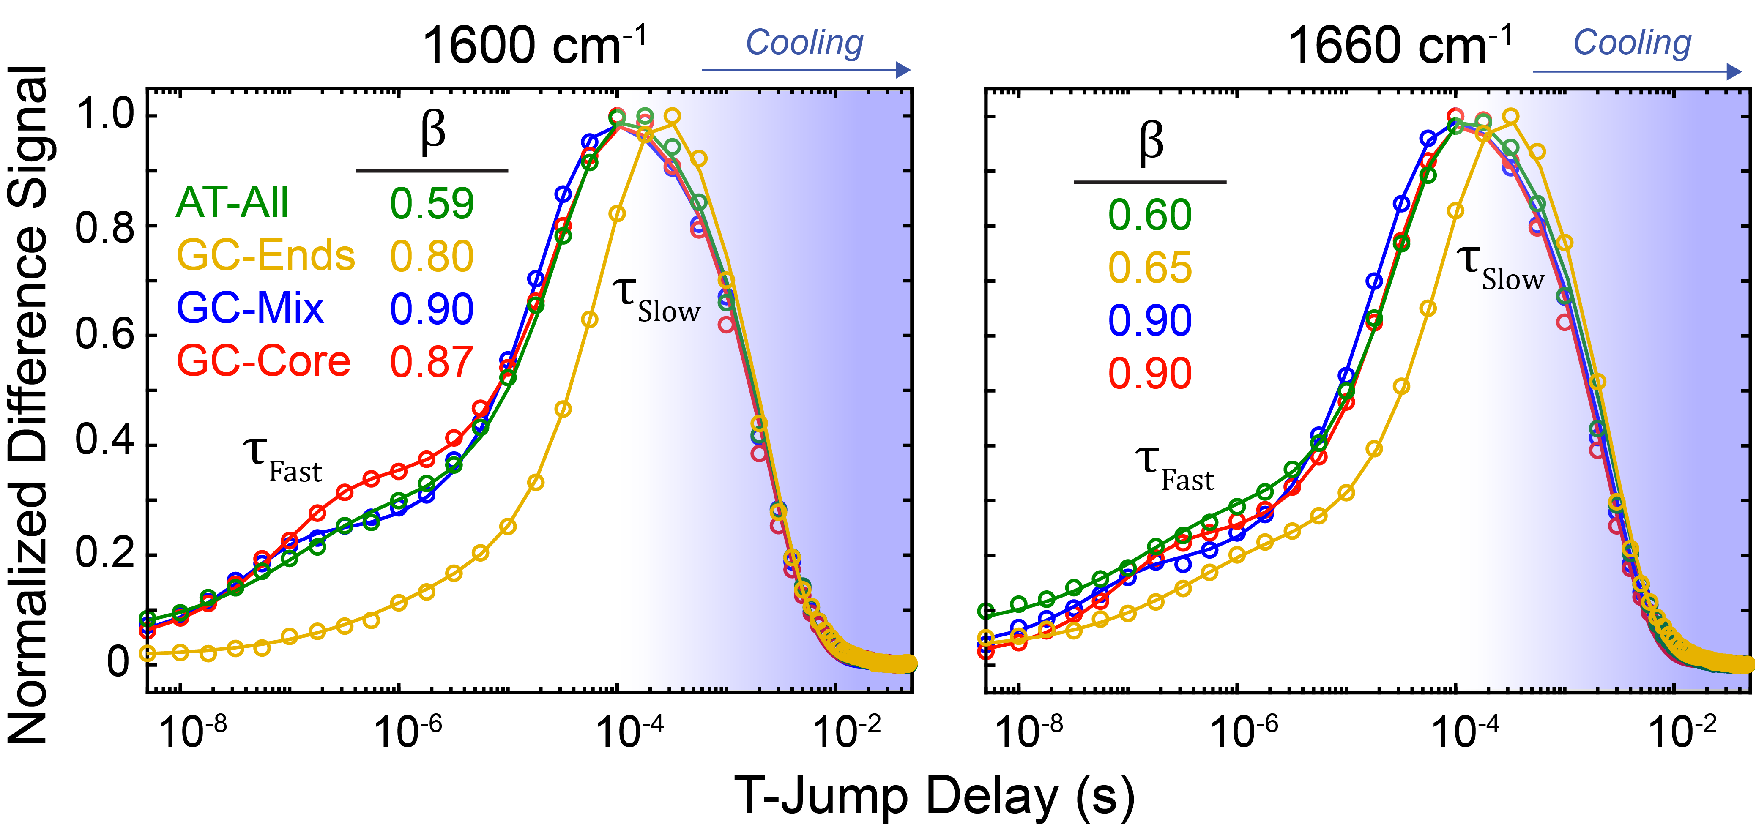
\includegraphics[width=150mm, scale=1]{Fig6.pdf}
        \caption{Normalized time traces from T-jump HDVE data probing the change in in-plane nucleobase vibrations. The signal at 1600 cm-1 corresponds to A and T nucleobases while the signal at 1660 cm-1 contains G, C, and T contributions. Each T-jump was performed with a temperature change of 15 °C to a final temperature near the Tm of each respective sequence. Each time trace was fit to the sum of a stretched exponential and two exponentials (solid lines). The stretched exponential describes the component from 10 ns to 1 μs ($tau_{Fast}$), and the two exponentials describe the signal rise from 1 - 300 μs ($tau_{Slow}$) and thermal relaxation of the sample back to the initial temperature. The stretch factor (β) from each fit is listed.}

        \label{fig:Fig6}
	\end{center}
\end{figure}

In addition to identifying relaxation timescales, the T-jump IR response profile can inform the distribution of dynamics contributing to the response. In particular, the fast response of AT-all and GC-end exhibits more stretched exponential character than for GC-core and GC-mix  (Figure \ref{fig:Fig6}). Furthermore, the GC-end response contains both G:C and A:T vibrational contributions, suggesting that native terminal base fraying may not be the unique source of the response. On the other hand, GC-mix and GC-core are characterized by a distinct fast response comprised only of A:T features that points to A:T fraying as the predominant dynamic source. We predict that the mid-IR responses of fraying and shifting are not clearly distinguishable for GC-ends and AT-all, therefore we cannot determine the stretched responses originate from fraying dynamics in out-of-register configurations, shifting mechanisms during the dissociation process, or some combination of the two. Although reproducing stretched signals is not within the scope of this analysis, we see qualitative agreement between more complex transition network (AT-all > GC-end > GC-core ~ GC-mix) and increased stretching in the fast response. 

% We expect that fraying would still occur in out-of-register conformations but at a different rate than intact fraying.

%It is difficult to distinguish a collection of different starting configurations -- such as out-of-register duplexes -- and their associated dynamics prior to the temperature jump from mechanistic pathways after the jump.

%We emphasize that this does necessarily reflect shifting relaxation timescales themselves but more likely changes in the fast responses -- e.g. fraying out-of-register -- within the collection of metastable states. 

\subsection{Centralizing GC placement induces long-lived, kinetically relevant fraying} % not sure if I should make this its own section?

The GC-core sequence represents a departure from the dominant shifting dynamics observed for AT-all and GC-end. Instead, the dynamical analysis describes a hybridization/dissociation pathway facilitated by a unique, highly frayed state (F4). Previous studies suggests that once key native contacts are made, the zippering mechanism ensures that the helix will quickly form outward \citep{Romano2013DNADependence, Yin2011KineticsHybridization}. Our results indicate, however, that the relative instability of A:T bonds compared the GC core can interrupt this process and form a longer lived metastable state. This occurs during the dissociation process as well, where one half of the A:T base contacts are entirely broken for a substantial period of time before the full dissociation event occurs. We observe these events to occur with equal probability on either permutable end of the helix. 

The F4 state is more accessible from an already bound helix, and once oligos are in F4, they are over 20x more likely to return to H than to D. Thus once a D $\leftrightarrow$ F4 transition has occurred, a F4 $\leftrightarrow$ H transition will likely proceed. On the other hand, H $\leftrightarrow$ F4 events are more frequent but unlikely to initiate complete dissociation. We previously noted that frayed dynamics are substantially accelerated in the 3spn2 model, which may lead to the F4 state being sampled more frequently then in experiment. Because GC-core stability is most sensitive to fraying, this effect could cause GC-core to dissociate more frequently and lead to the deviation in slow response we note in figure 2.

% discuss computational comparisons needs work
Lattice model studies have shown that frayed intermediates make substantial contributions to the GC-core conformational ensemble \citep{Araque2016LatticeCooperativity, Phys2019,Sanstead2020OxidizedDNA}. Araque et al. defines a similar 8-mer sequence (dATGCGCAT) as non-two-state, where a stable, symmetrically A:T frayed state is a crucial part of the duplex transition path \citep{Araque2016LatticeCooperativity}. When examining all four sequences using T-jump IR and 2D IR spectroscopy, Sanstead et al. found that the GC-core had the highest deviation from two-state behavior during dissociation (when excluding out-of-register contributions) \citep{Sanstead2016}. As T-jump IR data only showed a loss of A:T contacts during the fast response, this intermediate state was defined by a high degree of fraying about the central core. While 1-2 base pair fraying was commonly observed for GC-mix and AT-all as well, lattice model predictions showed that GC-core had substantially more frayed base pairs \citep{Phys2019}. Variable T-jump measurements and Smoluchowski simulations on model 1D free energy landscapes showed that AT termini fraying was an effectively barrierless process characterized by rapid inter-conversion between all accessible frayed states \citep{Sanstead2018DirectDehybridization}. We see the same rapid fraying in simulation data -- which is too fast to be attributed to a converged SRV mode -- however our SRV-MSM results show this inter-conversion first relies on the slower formation of the the A:T bond nearest to the GC center.  Although this process occurs much slower than single A:T base bonding and breaking, it may be difficult to experimentally discern from the overall hybridization process which contains both G:C and A:T character and occurs on a similar timescale.

%Our diffusion map analysis further shows how the ensemble of 4-bp frayed configurations impede helix formation.

\begin{figure} %[ht!]
	\begin{center}
	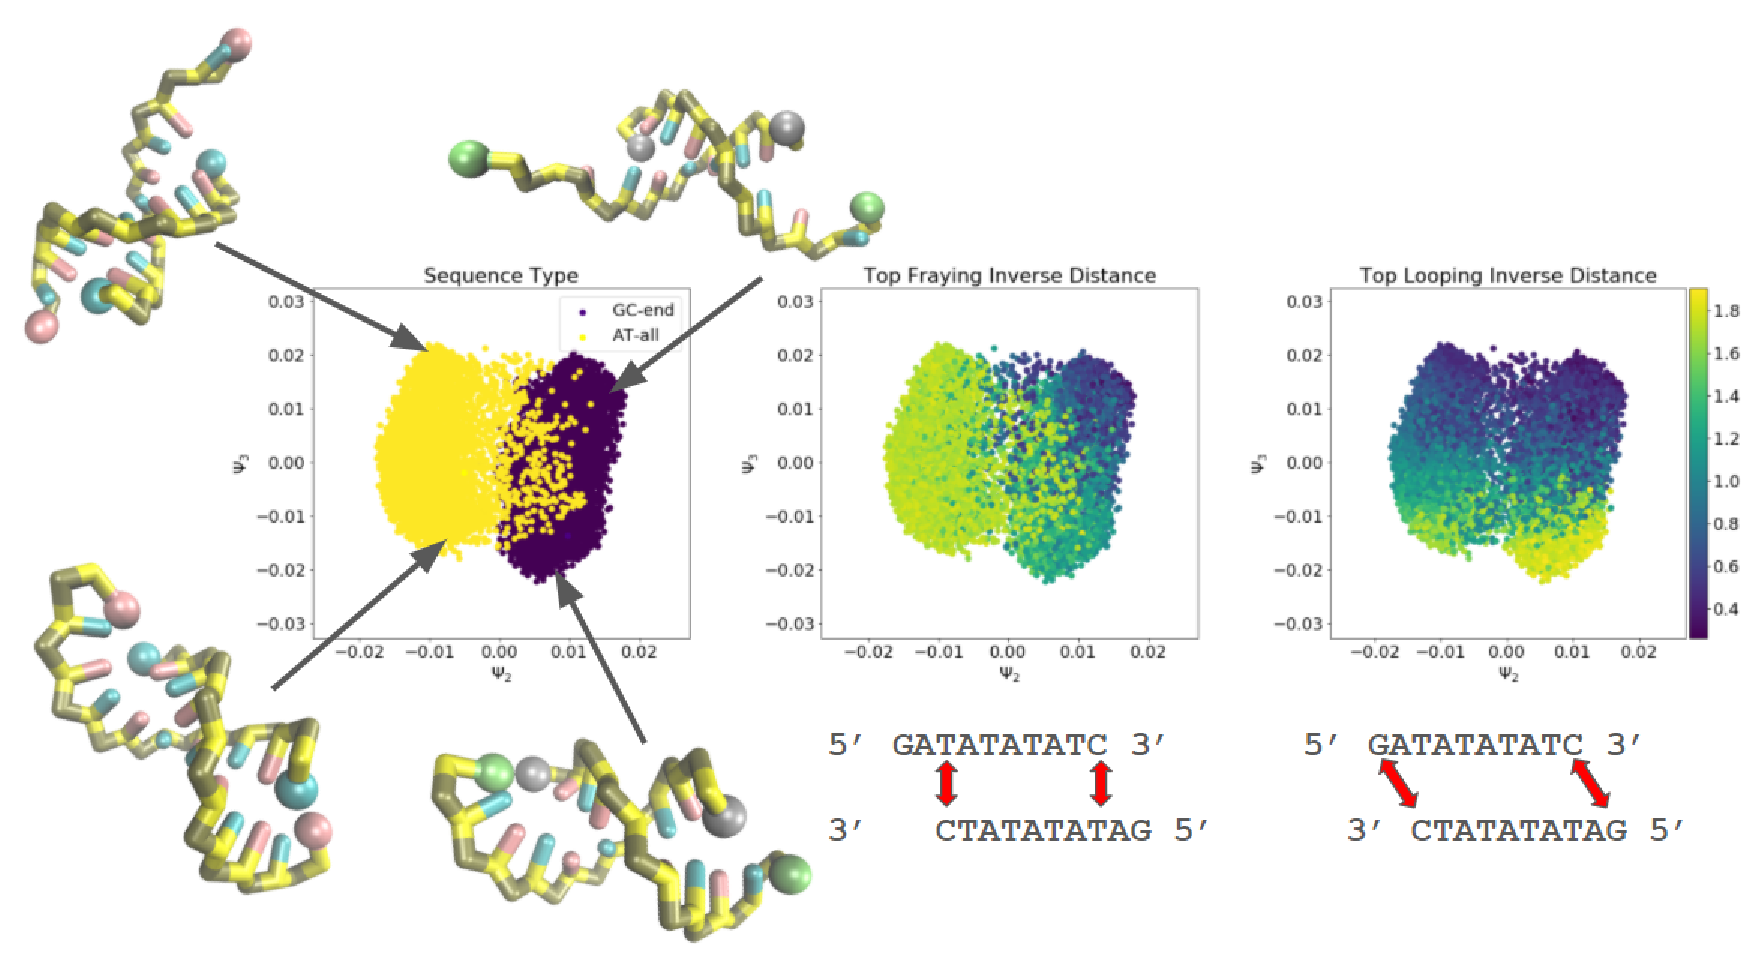
\includegraphics[width=150mm, scale=1]{Fig7.pdf}
        \caption{WC base pair distance and molecular renderings along two representative GC-mix hybridization and dissociation events. Permutable distances are reflected across the x-axis and show that fraying in the hybridized states tends to occur independently on either end of the duplex until fully dissociation occurs. The SRV-MSM state is shown along the x-axis, indicating the point at which a transition has been determined. Fluctuation between states is common during the transition.}
        \label{fig:GC-mix_transitions}
	\end{center}
\end{figure}

\subsection{Heterogeneous base pair distribution promotes nucleation-zippering hybridization and dissociation}

Given the lack of a repetitive AT interior (as in AT-all and GC-end) or exterior (as in GC-core), we expect more canonical dynamics from GC-mix. Although GC-mix dynamics are most similar to those of GC-core, we did not observe a converged slow mode corresponding to multi-base fraying behavior for GC-mix. Instead, we observed two modes converge, corresponding to the association/dissociation dynamic and diffusive behavior while strands are dissociated, respectively. Given that this second mode did not inform the hybridization process, we designated this transitions as effectively two-state within the resolution of our model. We did, however, observe substantial fraying of the two AT termini in the simulation data. Although these frayed states may be too short-lived to resolve a distinct slow mode, this behavior shows qualitative agreement with experimental analysis of this sequence which attributed fraying prior to dissociation as a deviation from all-or-nothing behavior \citep{Sanstead2016}.  While AT-termini fraying is surely a prerequisite to dissociation, we find these states to be so common and fleeting that very few progress to full dissociation compared to the F4 state. Furthermore, one or two base pair fraying does not fundamentally disrupt the helix in such a way that its re-formation is kinetically inhibited by the intermediate structures we present for GC-core.  

To supplement GC-mix analysis, we looked at qualitative trends in our trajectory data near hybridization and dissociation events, paying close attention to the distances between matching WC-pairs (Figure \ref{fig:GC-mix_transitions}). During hybridization, we observed the formations of some key base pair contacts before the full duplex formed. Specifically, first contacts tended to involve one of the G:C bonds and at least one neighboring A:T. This behavior is indicative of a nucleation-zippering mechanism as has been reported in previous studies \citep{Wetmur1968KineticsDNA, Porschke1971CooperativeTransition, Yin2011KineticsHybridization}. For dissociation events, we noted two base pair fraying on one or both sides of the duplex followed by more rapid dissociation of the central base pairs. There's evidence of a short-lived state composed of 2-4 base pair contacts immediately before full dissociation occurs. In contrast to the F4 state we observe in GC-core, these conformations do not form a distinct free-energy minima in SRV or tICA space, nor do they tend to reform intact duplexes. As a whole, these dynamics are similar to previously reported "fraying-peeling" mechanism \citep{Wong2008TheSimulations, Perez2010Real-timeUnfolding, Zgarbova2014BaseRNA}. We observed similar fast dynamics and transition states in the other three sequences, however they are more difficult to discern as they occur in concert with the longer lasting metastable states discussed above.


\begin{figure}[ht!]
	\begin{center}
        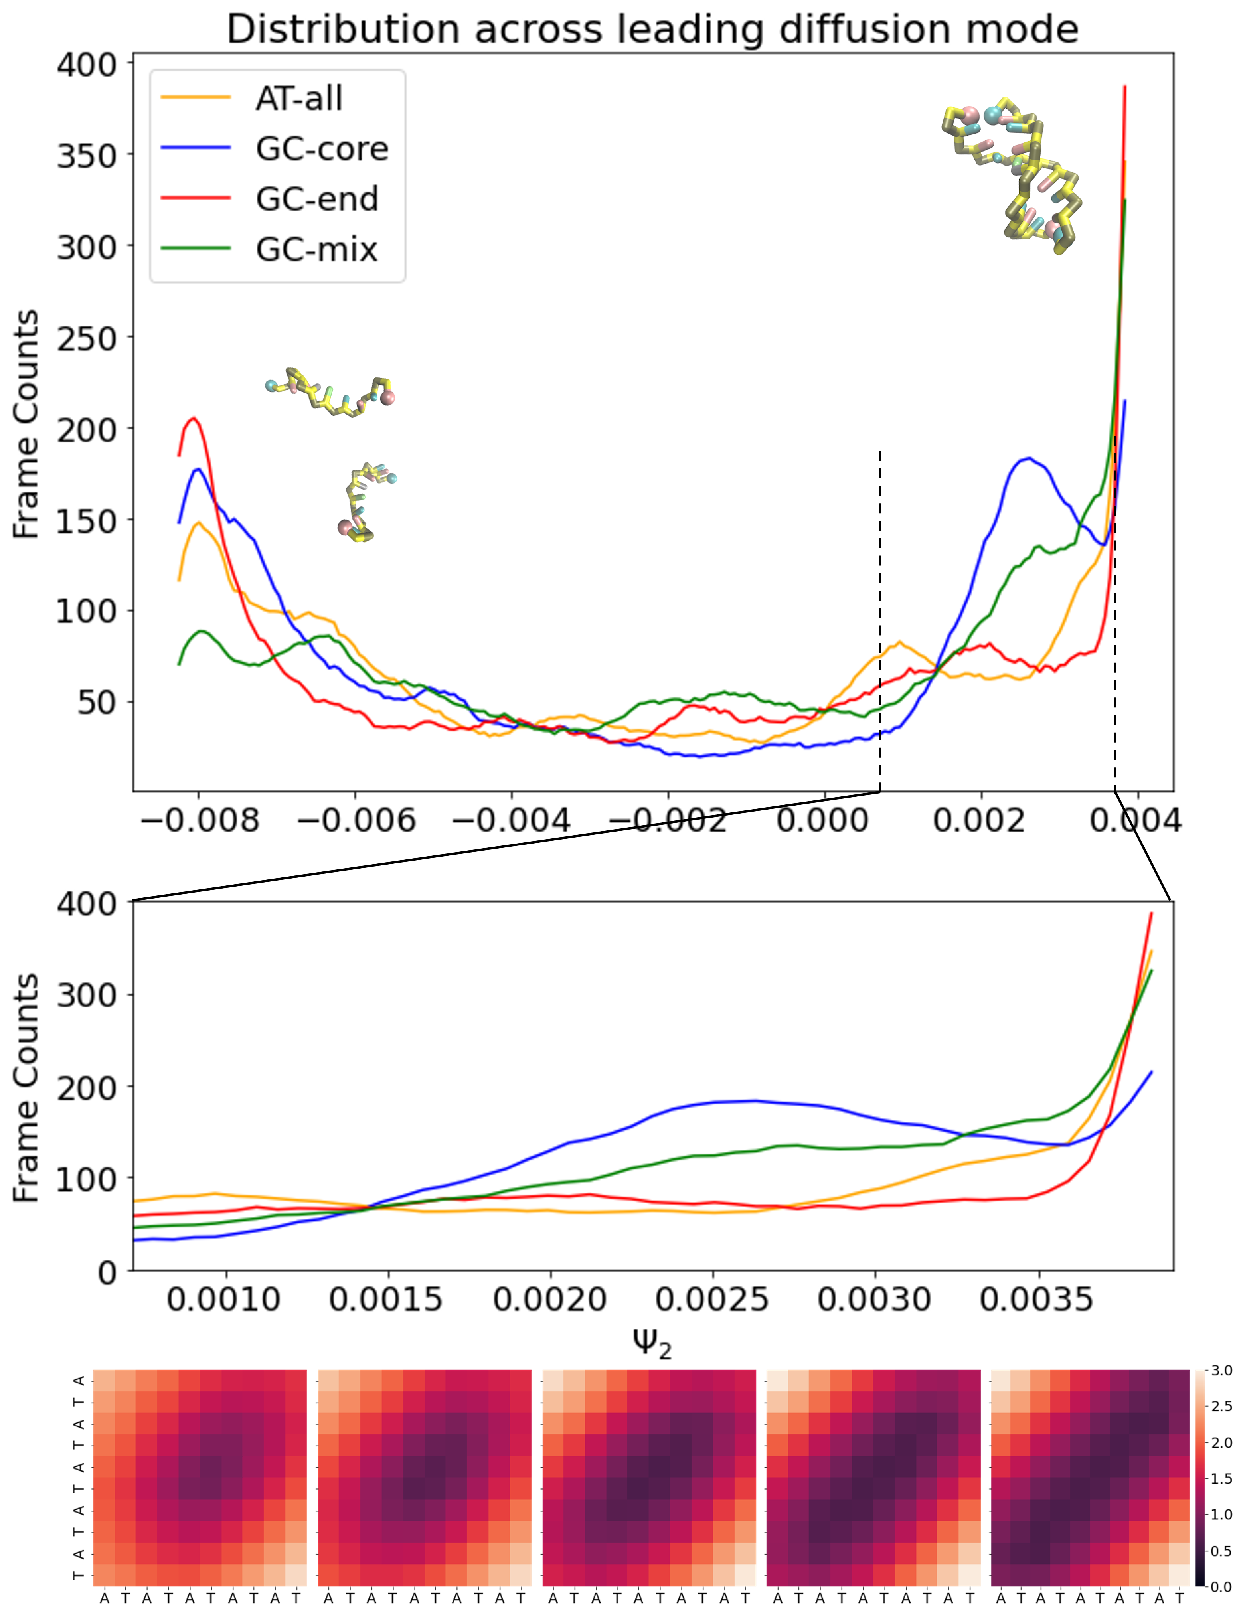
\includegraphics[width=150mm, scale=1]{Fig8.pdf}
        \caption{First two diffusion map coordinates built from 10000 5S1 states, equally sampled from AT-all and GC-end. Color maps show inverse distances (nm$^{-1}$) between out-of-register ends and complementary ends. The lower right region of the diffusion map space shows a high concentration of "shifted loop" base pairs that may facilitate the out-of-register GC-end transition.}
        \label{fig:GC-end_dmaps}
	\end{center}
\end{figure}

% need to gear this more towards the kinetics
\subsection{5s1 state distributions reveal differences between AT-all and GC-end kinetics}

Although our SRV-MSMs provide useful insight into slow processes, we were also interested in the ensemble of configurations within PCCA+ macrostates and during transition periods. These configurations interchange significantly faster than the SRV and MSM lag times, but we can use a diffusion map embedding to glean a structural understanding of the macrostate population. Diffusion maps generate a low dimensional embedding of the data into high variance structural modes and are well-suited to find subtle differences in temporally disconnected data \citep{Coifman2006DiffusionMaps, Ferguson2010SystematicMaps}.

While examining molecular renderings, we noticed that a significant proportion of GC-end 5s1 configurations retained one native G:C bond, even when all available A:T bonds were formed out-of-register. We would not necessarily expect duplexes to sacrifice helical conformational entropy in order to facilitate termini bonding. To compare how these state populations differ between GC-end and AT-all, we employed diffusion maps built on an equal sampling of 5000 conformations from the 5S1 state of both sequences. We used all 100 intermolecular distances (as opposed to the 55 permutation free coordinates used to construct SRV-MSM) as our distance metric, making it easier to discern structures that form on either permutable end of the shifted conformation. This created degenerate 2nd and 3rd diffusion modes, with nearly equal eigenvalues, differentiating effects at the identical "top" and "bottom" of the strands. In Figure \ref{fig:GC-end_dmaps} we present the first two non-trivial diffusion map eigenfunctions and show representations of the degenerate third coordinate in the SI (Figure \ref{fig:GC-end_dmaps_full}). Diffusion maps built from samples of the 3S1 states are also shown in the SI (Figure \ref{fig:GC-end_dmaps_3prime}). 

The first diffusion mode clearly delineates between the GC-end and AT-all shifted conformations and correlates highly with the average distance between the 3' end and its shifted complementary pair. As expected, this shows that mismatched C:T pairs are never bound whereas the AT-all pairs are mostly bound with occasional fraying indicated by small AT-all overlap in the GC-end region. The second diffusion mode, which correlates highly with the average distance between 3' and 5' ends, highlights structural variances within the two sequences distributions. We notice that about 40\% of GC-end configurations fall below $\Psi_3 = -0.01$  compared to only 10\% of AT-all configuration. We find that these GC-end populations share stabilizing termini contacts despite all A:T contacts being shifting out-of-register. These "shifted-loop" bonds appear uniquely stable for GC-end conformations,  and suggest an intermediate states through which hybridization is facilitated. This may account for the GC-end 5S1 $\rightarrow$ H transition being more favorable than  5S1 $\rightarrow$ D despite the state free energy being substantially higher than the AT-all equivalent.

%This effect may be exaggerated given that C and T base pairs are assigned slightly higher excluded volume radii in 3spn2 \citep{Hinckley2013AnHybridization}. 

%Although AT-all shifted ends tend to stay bound out-of-register, the second diffusion coordinate shows some population of inert tails that fold back onto the helix. 

% need to work on this if adding to this section (might belong somewhere else or not at all?
%Although internal base pair mismatches can cause substantial conformational distortions such as kinking, terminal mismatches have been shown to be slightly stabilizing and have a minimal effect on helical character \citep{Santalucia2004TM, DiMichele2014EffectHybridization}. In the context of the 3spn2 model, these ends are accounted for via intra-strand base stacking and inter-strand cross-stacking interactions \citep{Hinckley2013AnHybridization}. The only direct interaction between non Watson-Crick (WC) basepairs is parameterized by isotropic excluded volume potential, which is likely more simplistic than the true mismatch interaction. 

%AT-all looping could be a consequence of multiple bps sharing the same wc partner (I believe this is possible in 3spn2, because types of bonds are only mutually exclusive between cross-stacking, bp binding, and excluded volume)%

\subsection{Sequence-dependent fraying determines direct hybridization pathways} 

\begin{figure}[ht!]
	\begin{center}
        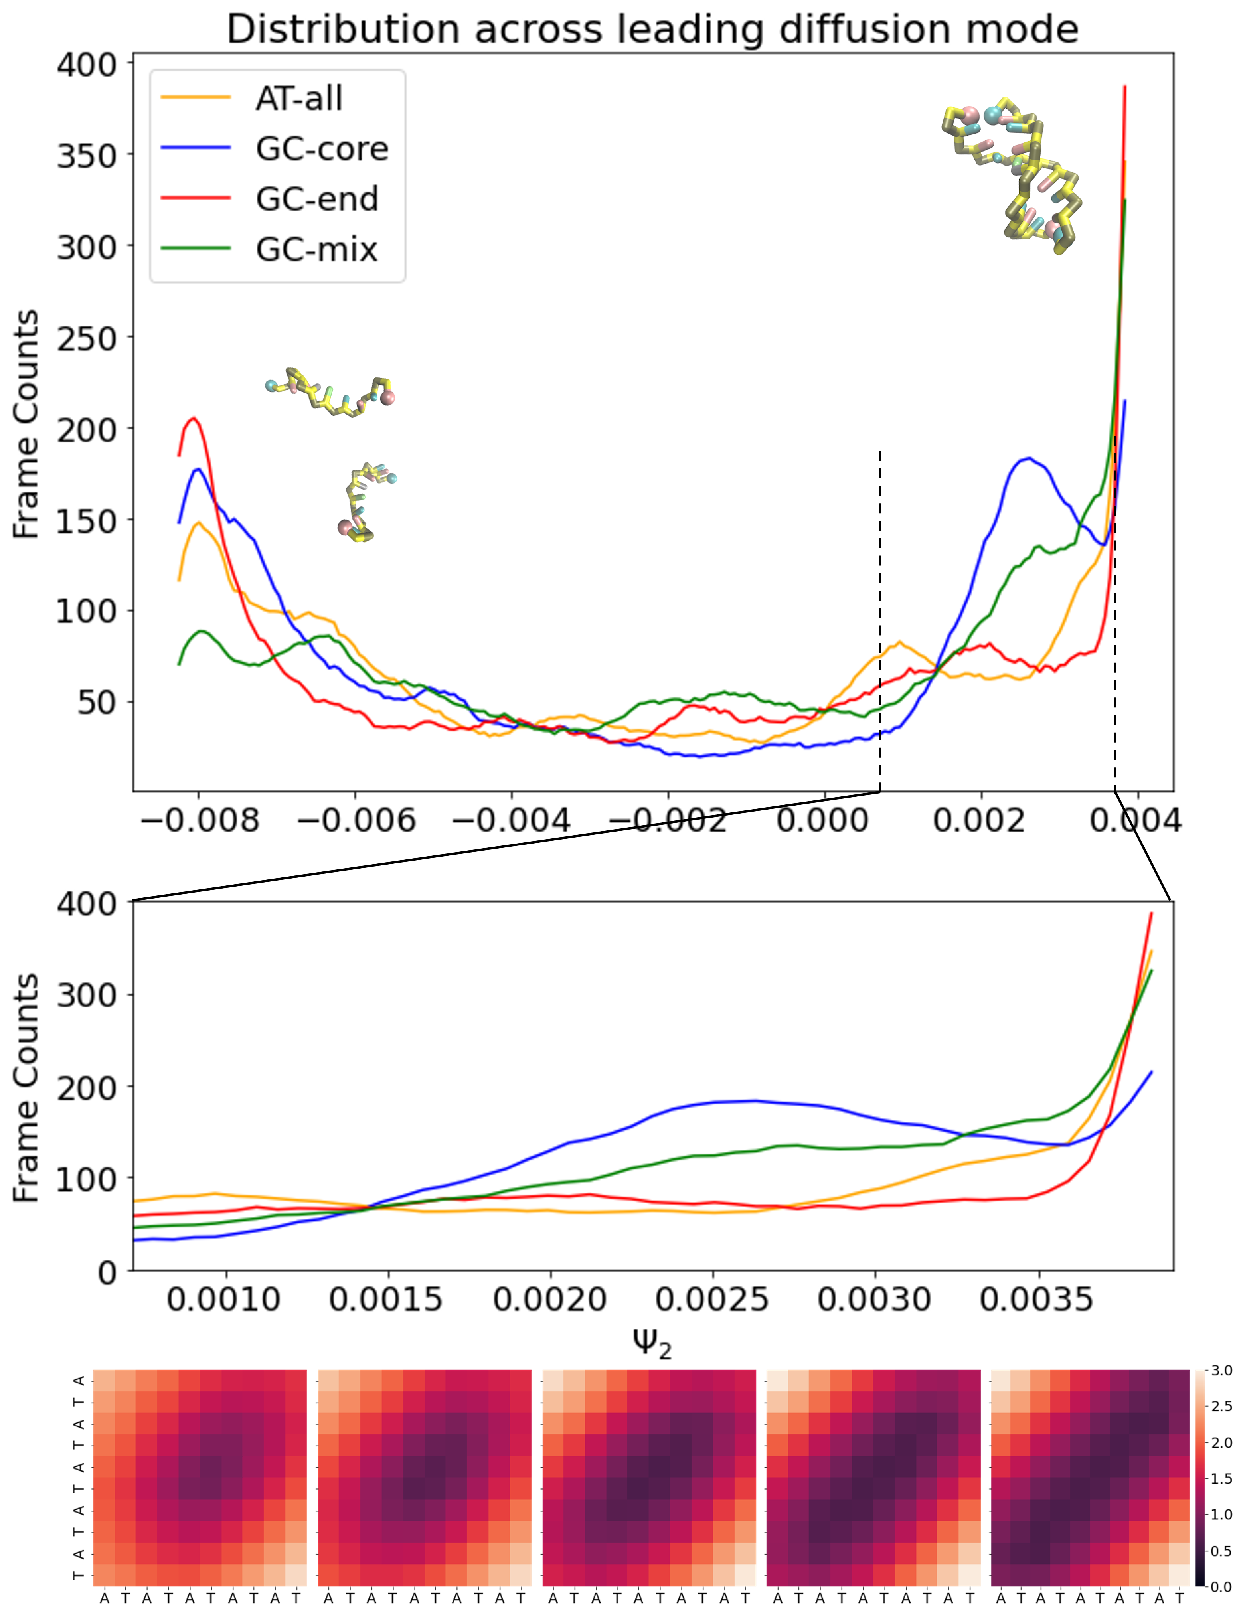
\includegraphics[width=150mm, scale=1]{Fig9.pdf}
        \caption{Sequence-dependent population distributions for trimmed hybridization events. $\Psi_2$ represents the maximum structural variance across all sequence configurations and correlates strongly with hybridization progression. Populations are discretized in 200 bins and smoothed by averaging with the nearest 5 bins. Heat maps show the average intermolecular base distances in nm at increasing values of $\Psi_2$, where the main diagonal shows native base pair distances.}
        \label{fig:Fig8}
	\end{center}
\end{figure}

(I just completed most of this analysis on Friday. I think this shows a more direct comparison to Paul's 2016 kinetic model -- mainly all-or-nothing deviations caused by fraying are ordered GC-core > GC-mix > AT-all > GC-end. In addition we see a distinct state form for GC-core which serves to verify the F4 state and its kinetic relevance. Lastly it provides another means by which MSMs can inform analysis techniques for clearer comparison between sequences. I could repeat this procedure and analysis for direct dissociation as well if that is of interest)

To more directly compare fast hybridization dynamics across all sequences, we trimmed simulations centered on direct D$\rightarrow$H (or D$\rightarrow$F4$\rightarrow$D for GC-core) events and excluded transitions that passed through long-lived out-of-register states. To achieve higher resolutions, we reran simulations with a 10x higher save rate and selected a 1000 frame region (10 ns simulation time) for each event. We built diffusion maps on a set of 48 such "trimmed" events evenly sampled across sequences. We found a distinct spectral gap after the first non-trivial diffusion map eigenvalue, indicating that the leading mode $\Psi_2$ contained most of the structural variance. Indeed, we found $\Psi_2$ had a 0.89 Pearson correlation with simulation time and a  -0.94 correlation with inter-strand core distance with minimal variation by sequence. This shows that $\Psi_2$ is strongly correlated with hybridization progress for all sequences and represents a consistent collective variable for comparison between sequences. 

Once we determined a strong hybridization coordinate, we compared probability distributions for each sequence along $\Psi_2$ (Figure \ref{fig:Fig8}). The $ <\Psi_2 < 0$ reflects the distance between approaching strands, but we noted statistically meaningful differences between sequence once first WC contacts are made. In the $ 0.001 <\Psi_2 < 0.0035$ region, heatmaps show that contacts tend to form near the center of the duplex, and frayed structures progressively zipper closed as $<\Psi_2$ increases. As expected, GC-core shows a distinct peak in the frayed region, corresponding to the F4 macrostate identified by SRV-MSMs. GC-mix has a notably higher population than AT-all and GC-end but displays a more gradual progression toward the native hybridized state. This is consistent with the downhill nucleation-zippering mechanism described above. Although differences between AT-all and GC-end are more subtle, overall sequence populations in this region follow predictions by Sanstead et. al. regarding deviations from two-state binding behavior, where GC-core > GC-mix > AT-all > GC-end \citep{Sanstead2016}. This qualitative agreement shows that MSM information can be adapted to compare sequences along common pathways and elucidate dynamics occurring faster than the lag time. Furthermore, we are able to distinguish out-of-register deviations from fraying deviations and describe relevant experimental comparisons for each.

%This time, we set our distance metric to the same permutation-free coordinates we used to build the SRV-MSMs. 

% add new info here, not sure if shifting discussion is necessary
% take away message is that these are good proxies for the responses
% although there is not perfect agreement, we show that these are very reasonable coordinates assing fast and slow response


\subsection{Limitations}

Although we were able to obtain improved resolutions on several relevant dynamics by using a shared lag time across sequences, we found it difficult to converge relevant faster processes such as duplex nucleation and zippering. These processes are crucial to duplex formation, however they do not appear to be kinetically metastable or slow relative to other timescales of interest. Furthermore, they can initiate at various points along the strand, which, under out present featurization method, may appear as a collection of modes instead of as one distinct process. We also found the need to strike a balance between adequate sampling of hybridization events and frame save rate in order to maintain tractable SRV-MSM calculations. Indeed, we collected over 10 GB of equilibrium trajectory data for each sequence, and were working near memory limits when training SRVs and building SRV-MSMs.

In any high-level model there are inevitable simulation artefacts produced by coarse-grained approximations. For example, the treatment of non-interacting base pairs as an excluded volume potential alone may not be representative of dynamics produced from mismatched dangling ends. In general, coarse-grained models produce a smoother free-energy surface which can results in much faster motions between states. This is illustrated by substantial accelerations in temperature-dependent responses when compared to experiment. Furthermore, it may be easier to cross between states -- e.g. a 5S1 $\rightarrow$ H transition -- when the usually rough free energy path becomes more easily traversed. 

\section{\label{sec:conc}Conclusion}

We have demonstrated how G:C placement in an otherwise repetitive AT sequence has a profound impact on equilibrium hybridization dynamics. By supplementing coarse-grained MD with data-driven time-lagged analysis, we constructed high resolution SRV-MSMs capable of distinguishing sequence-dependent kinetic behavior. In particular, we found that AT-all and GC-end sequences both participate in some degree of out-of-register base pair shifting, although these states have higher kinetic relevance for AT-all. On the other hand, GC-core hybridization transits through, or is perhaps facilitated by, a frayed intermediate in which one half of A:T bonds are broken and the duplex is significantly disrupted. Our computational approach and results show strong comparisons T-jump experiments at ns and us timescales. Going forward, we expect that this work will be extended to predict more general trends in sequence-dependent hybridization and motivate strategies for experimental comparisons. These insights should be leveraged for sequence design and incorporated into the growing field of dynamic DNA nanotechnology. 

\newcommand{\sectionbreak}{\clearpage}
\section{\label{sec:Results}Supplemental Information}

% add secion on dmap and high temp methods?
%\subsection{Additional methods}

\begin{figure}[ht!]
	\begin{center}
        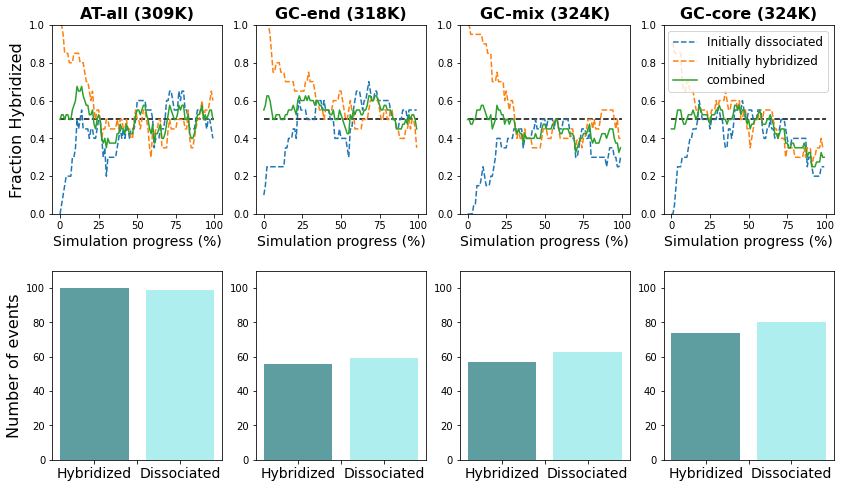
\includegraphics[width=120mm, 
        scale=0.5]{Figs/figs_imp/allseq_event_count.png}
        \caption{All sequences consist of 20 trajectories initialized in the hybridized states and 20 in dissociated state. The fraction of hybridized duplexes averaged across these sets is shown over time. For all sequences these curves converge near 0.5, but stochasticity of rare-event makes a definitive Tmelt difficult to identify. The number of hybridization/dissocation combined across trajectories is shown. Not every trajectory contained a transition event, but on average more than one full event occurred (H$\rightarrow$D$\rightarrow$H) per trajectory, providing adequate sampling of dynamics. AT-all undergoes substantially more transition, but many of these do not reach a native (in-register) hybridized state.}
        \label{fig:allseq_event_count}
	\end{center}
\end{figure}

\subsection{VAMP-2 Scoring}
The VAMP-2 score uses the covariances of a set of inputs to estimate the transfer operator of a dynamical system, providing a robust and object means to evaluate various parameters and models. Hyperparameters, including feature choice, number of microstates, and number of slow modes were evaluated and selection with via the VAMP-2 score. In the equations below, we show how covariances are obtained from some featurization $\chi$ of a time series $x_t$ and its time-lagged pairs $x_{t+\tau}$. The VAMP-2 score can then be found for $\chi$ by applying the VAMP principle with cross-validation.

\begin{align*}
 	\mathscr{C}_{00}=&\Expect{\chi(x_t)\chi(x_t)^\intercal}_t\\
 	\mathscr{C}_{01}=&\Expect{\chi(x_t)\chi(x_{t+\tau})^\intercal}_t\\
 	\mathscr{C}_{11}=&\Expect{\chi(x_{t+\tau})\chi(x_{t+\tau})^\intercal}_{t+\tau}\\
	\\
 	VAMP-2[\chi]=&\norm{\mathscr{C}_{00}^{-1/2}\mathscr{C}_{01}\mathscr{C}_{11}^{-1/2}}_F^2 +1
 	%VAMP2^{val}[\chi]=&\norm{\mathscr{(C_{00}^{val})}^{-1/2}\mathscr{C}_{01}^{val}\mathscr({C}_{11}^{val})^{-1/2}}_F^2 + 1
\end{align*}\label{CK1}

\subsection{SRV hyperparameters}

Using optimized hyperparameters and featurized trajectory data, we transformed 55 reciprocal pairwise distances into a low dimensional SRV basis set. In order to maintain consistency between sequences, we kept all SRV training hyperparameters the same with the exception of the number of outputed slow modes. We determined the number of slow modes via cross-validation on the VAMP-2 score to ensure that the coordinate did not over fit on statistical noise \citep{McGibbon2015VariationalKinetics}. In particular, we looked for convergence in the VAMP-2 score and inconsistency between cross validation scores -- suggesting that the model may be over-fitting on artifacts in the training data. We used a batch size of 50000 and ran each model for a total of 20 training epochs. We used two hidden layers and set the size of each layer to 100. For cross-validation and comparison between different hyper-parameters, we used a 80/20 validation split training. SRV training required about 22 GPU-minutes across 1 GPU and 10 CPUs. SRV training was implemented using Keras and Tensorflow \citep{KerasGithub.Com, Abadi2016TensorFlow:Systems}.

\subsection{SRV-MSMs provide better resolution than tICA-MSMs} 

\begin{figure}[ht!]
	\begin{center}
        \includegraphics[width=0.9\textwidth]{Figs/figs_imp/AT-all_implied_timescales.png}
        \caption{SRV-MSM implied timescales converged faster than tICA-MSM implied across the five leading AT-all modes. Timescales are directly compared at the chose lag time of 1.2 ns}
        \label{fig:AT-all_dynamic}
	\end{center}
\end{figure}
\begin{figure}[ht!]
	\begin{center}
        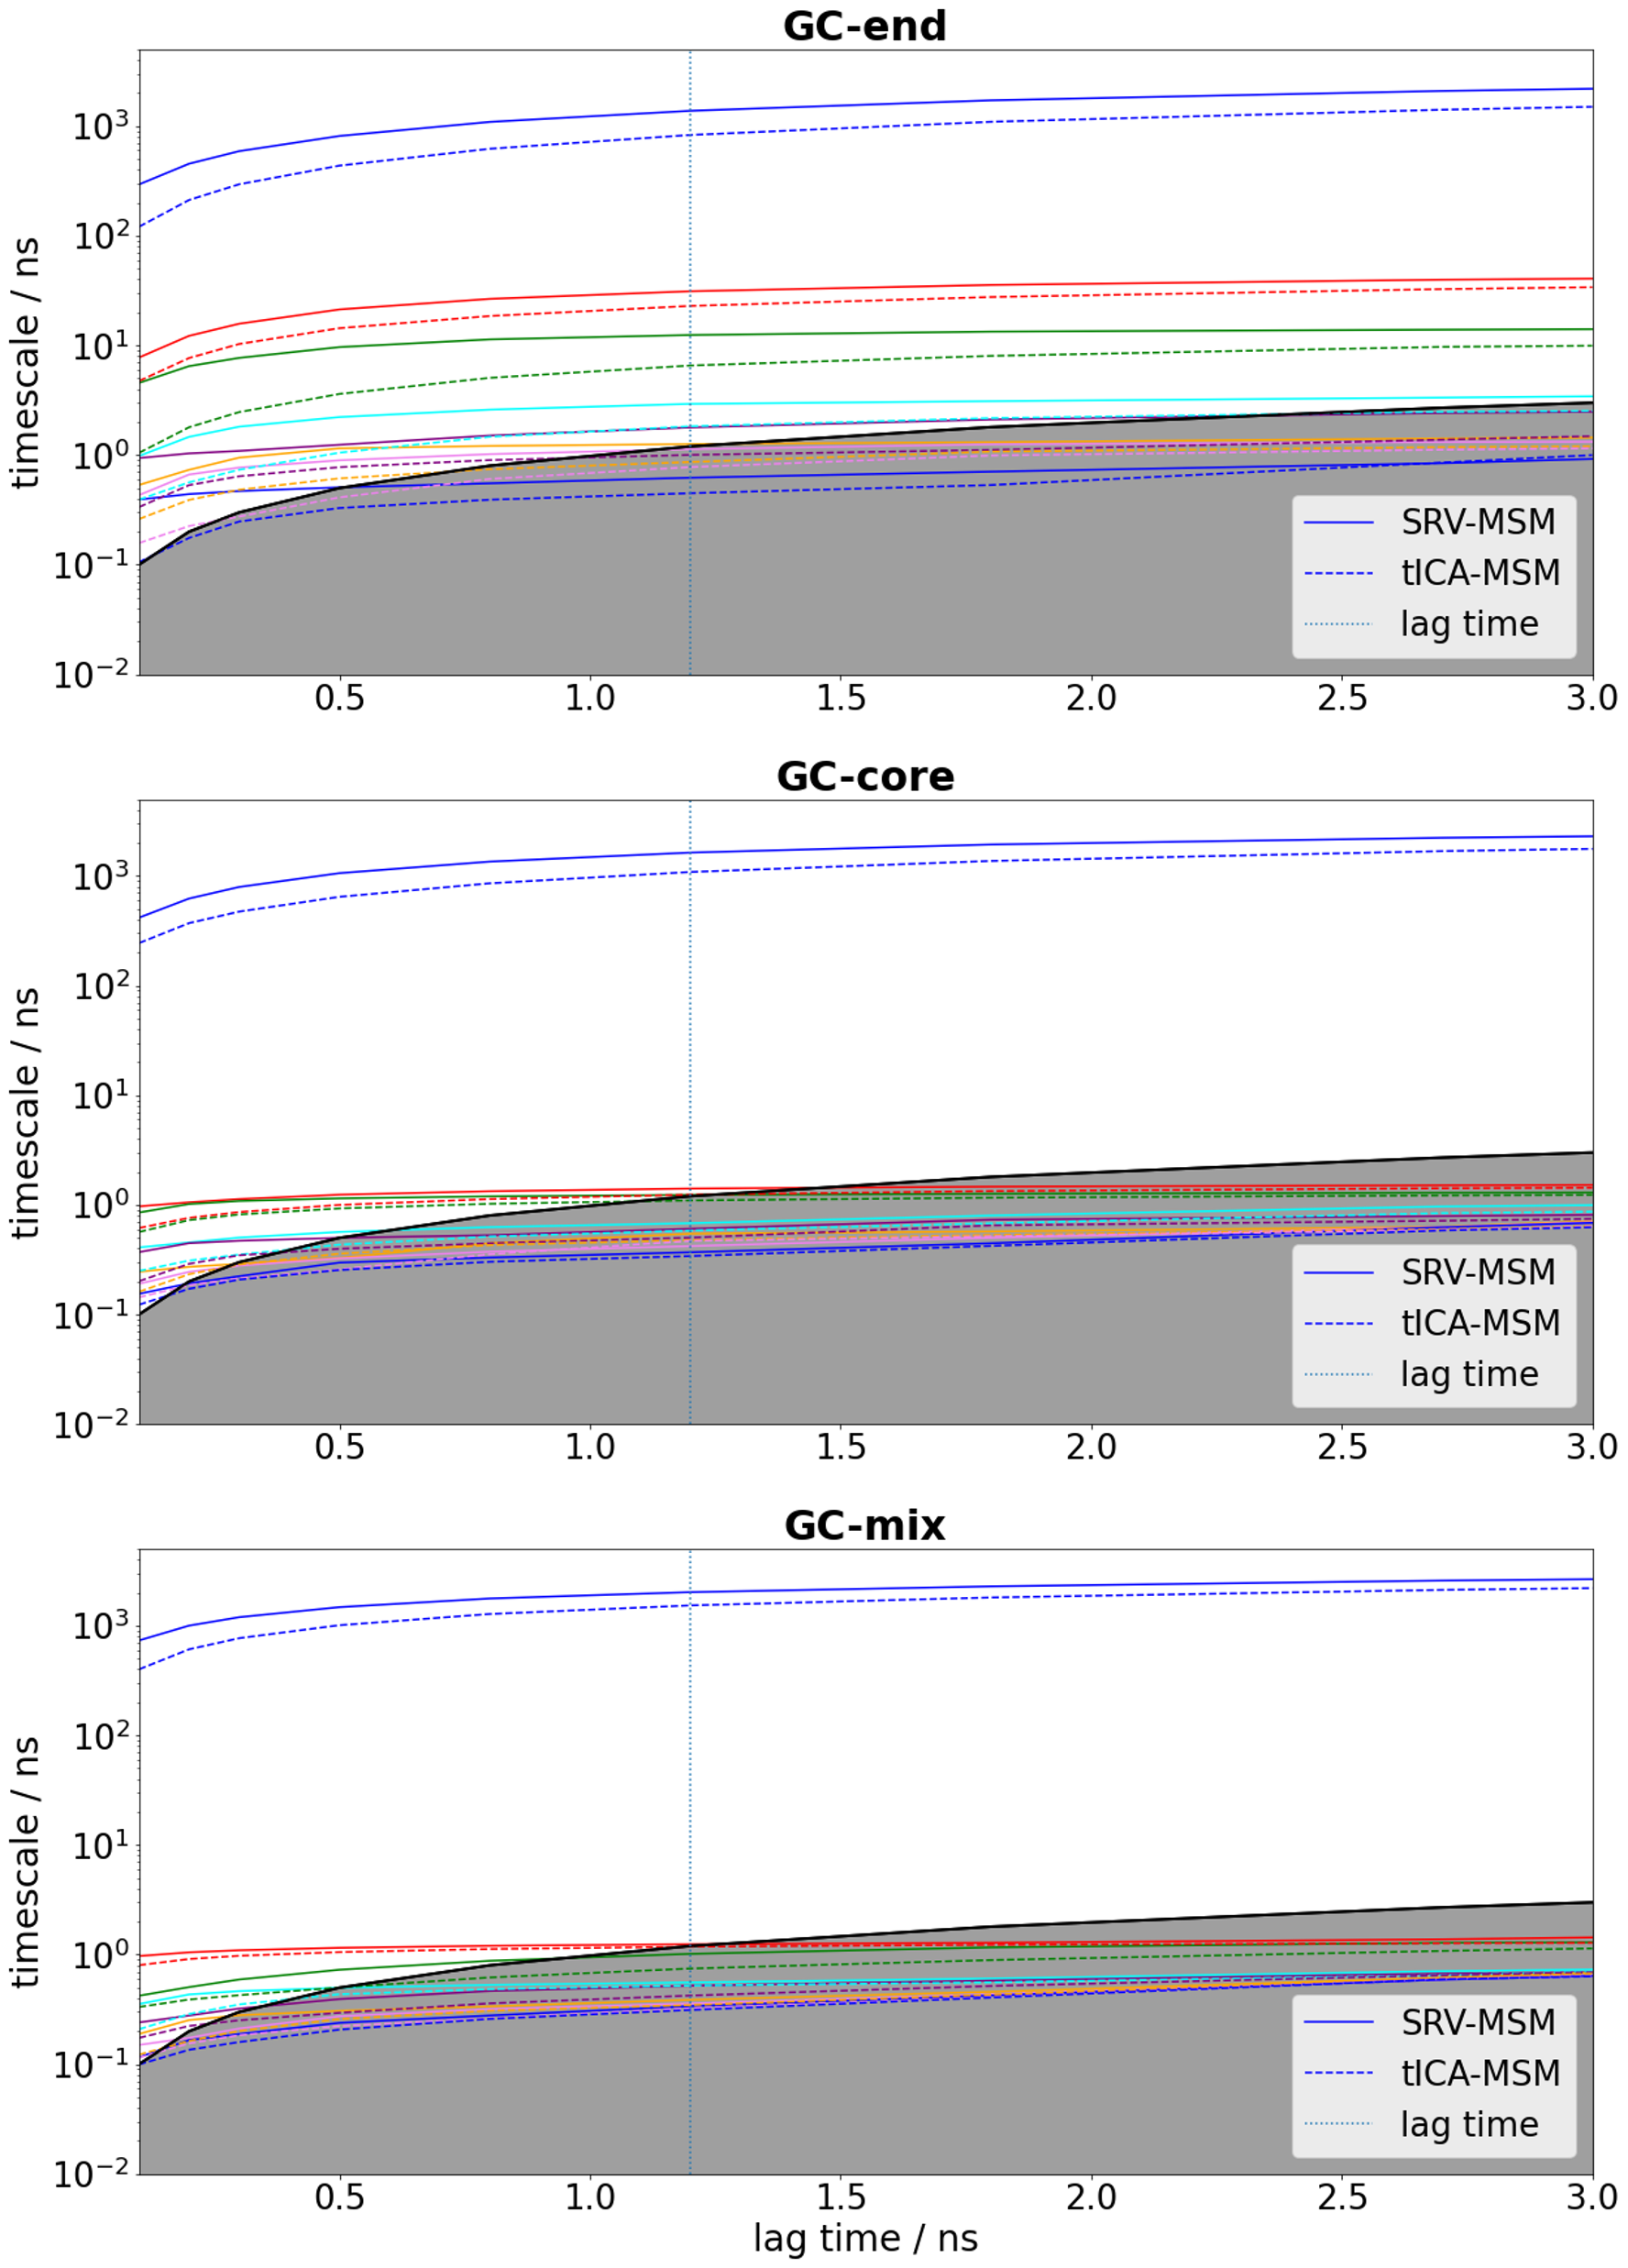
\includegraphics[width=80mm, 
        scale=0.5]{Figs/figs_imp/all_seq_implied_times.png}
        \caption{SRV-MSM vs. tICA-MSM implied timescales convergence for GC-end, GC-core, and GC-mix. Progressively larger spectral gaps are observed between the first mode and higher order modes. We observe convegenve of resolvable higher order modes at a shared lag time of 1.2 ns. It is difficult to converge the leading mode in this regime due to the infrequency of hybridization/dissociation events.}
        \label{fig:all_seq_lags}
	\end{center}
\end{figure}


\subsection{SRV-MSM walkthrough and analysis}
In our analysis, we found that the AT-all sequence, given its repetitive structure and lack of GC-content, produced the most discernable spectral gap between modes. For this reason, we use this sequence a case study to work through our SRV-MSM pipeline step-by-step. Our first task was to identify the SRV lag time that was longer than the intrinsic Markov timescales of the system, yet short enough to resolve the dynamics of interest \citep{Phys2018MarkovValidation}. We found that an SRV lag time of 1.2 ns showed good convergence across the relevant timescales for all sequences. Next we selected an optimal number of SRV components to include in our analysis. After a certain point, higher order dynamical modes provide diminishing contributions the overall kinetic variance as measured by the Vamp-2 score, and the model can begin fitting on statistical noise in the trajectory data instead of the true dynamics \citep{McGibbon2015VariationalKinetics}. It is also more difficult to perform kmeans clustering on a high dimensional space, especially when those higher dimensions are less kinetically relevant \citep{Pande2010EverythingAsk}. For these reasons, the number of slow SRV components should be carefully selected based on the specific system of interest. As shown in figure \ref{fig:allseq_srv_crossval}), we see diminishing returns in the VAMP-2 score after five slow modes and select these modes as our optimized SRV basis.

%\subsubsection{SRV-MSM construction and optimization}
Although SRV coordinates alone provide some information, we can access a more holistic picture of sequence kinetics and thermodynamics by using these SRV coordinates as a basis on which to construct an MSM. Because these coordinates are already capturing a majority of the system's kinetic variance, they serve as an ideal basis on which to group frames into microstates. We performed k-means clustering, and optimized the number of microstates at 200 by monitoring VAMP-2 score. Next, we selected an MSM lag time in a similar fashion to our SRV lag time selection process. This enables us to select a shorter lag time and build a higher resolution model than we could from an analogous tICA basis. Setting the MSM lag time to the same 1.2 ns we used for our SRVs, we built a Bayesian MSM to calculate transition probability matrix between each microstate. Finally, PCCA+ spectral clustering was implemented to group these microstates into macrostates that each represented a collection of metastable structures. Previous works have used a common set of microstates and/or performed manual clustering of microstates based on physical read outs from simulation data (stacking score, energies, etc) \citep{Pinamonti2017PredictingModels, PinamontiTheModels}. Although these techniques are useful for performing comparisons between sequences, we saw better results when optimizing MSMs to capture the most detail of sequence individually and thus developed an independent set of microstates and macrostates for each sequence. 

\begin{figure}[ht!]
	\begin{center}
        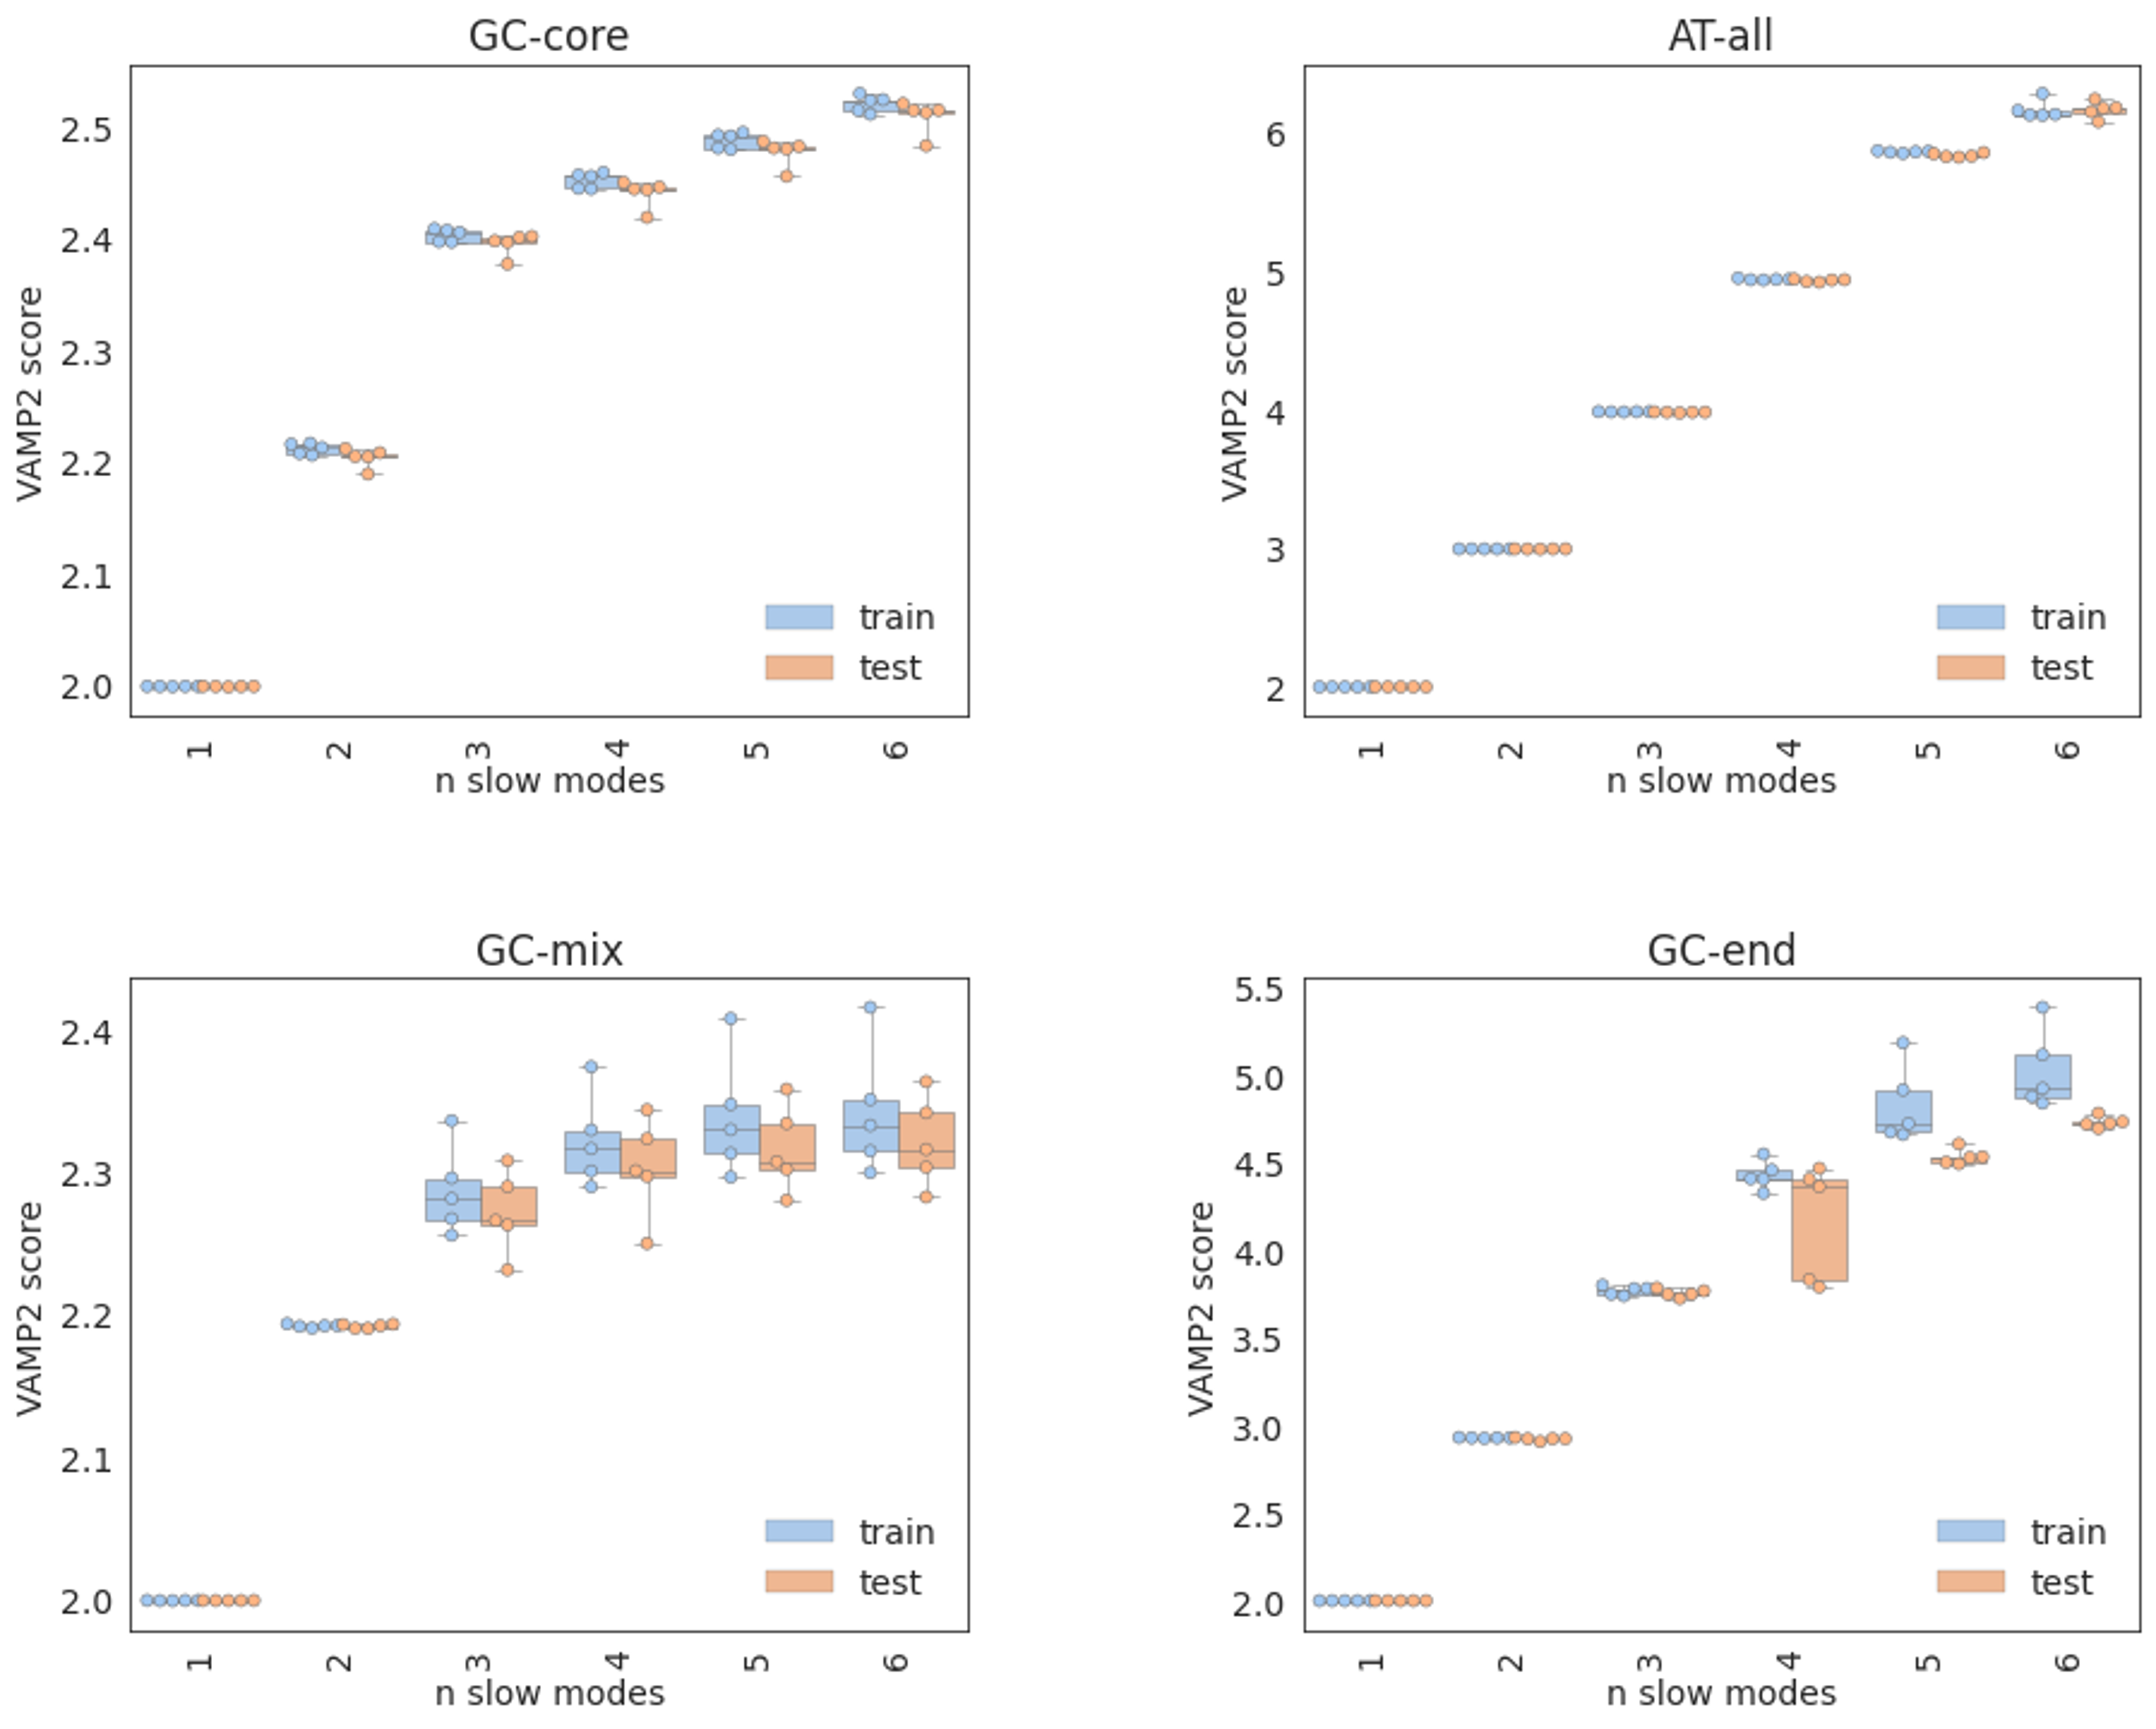
\includegraphics[width=120mm, 
        scale=0.5]{Figs/figs_imp/allseq_crossval.png}
        \caption{5-fold cross validation procedure to select number of SRV coordinates. We look for the converge of the VAMP-2 scores, inconsistent scores between folds, and deviation between training and test data as indicators that the model has begun fitting on statistical noise.}
        \label{fig:allseq_srv_crossval}
	\end{center}
\end{figure}

Next, we seek to interpret the physical relevance of these leading modes by plotting the Pearson correlation of each mode with the 100 intermolecular distances between strands. The quantitative meaning of these coordinates can be difficult to interpret given their nonlinear relationship to the SRV collective variables, but the relative different between these correlations shows which coordinates are most relevant to each process. For example, the first slow mode shows a positive correlation to each distance and the strongest correlation with native base pair distances (shown along the main diagonal). Given these correlations and the substantially longer timescale of this process, we can deduce that this leading mode corresponds to the overall hybridization and dissociation process. The next four SRV components all show a relatively high correlation along offset diagonals. These diagonals correspond to the intermolecular distances between complementary but out-of-register base pairs and point to the existence higher order "shifting" processes between sets of such base pairings. Previous "inchworm" and "pseudoknot" mechanisms have similarly been reported in simulation studies to correct base pair mismatches and occur on orders of magnitude longer timescales than underlying fast dynamics such as fraying \citep{Romano2013DNADependence, Markegard2015, Maciejczyk2014DNAModel}.

We found GC-end had a similar implied timescales distribution to AT-all, with a distinct spectral gap after the fourth mode. For AT-all and GC-end, we kept to the convention of clustering into n+1 macrostates, where n is the number of slow components captured by the MSMs. For GC-core we built an SRV-MSM using these first three SRV modes as a basis and proceeded along the pipeline as described above. We found that four macrostate clustering was unstable -- likely because the third mode is mostly providing  information about dissociation dynamics -- so we performed PCCA+ clustering into three macrostates representing the hybridized (H), dissociated (D), and 4 4 base pair frayed (F4) states.  The GC-mix sequence showed a similar implied timescale distribution to GC-core, however we no longer saw a converged slow mode corresponding to multi-base fraying behavior. Instead, we observed two modes converge, corresponding to the association/dissociation dynamic and diffusive behavior while strands are dissociated. These correlate closely with the first and third GC-core SRV modes. Although we built our SRV-MSM using these two coordinates, we again were unable to form a stable third state along the second coordinate. As such, we designated this transitions as effectively two-state within the resolution of our model.

%For GC-core and GC-mix, we found this clustering convention to be unstable -- likely because the last converged mode was providing information about dissociation dynamics -- and performed PCCA+ with one less macrostate. 

To visualize macrostates, we project the data into the two leading tICA coordinates. Although SRVs outperform these coordinates for the purpose of MSM construction, tICA coordinates represent good high variance collective variables on which to visualize free energies and state assignments \citep{Sidky}. Furthermore, we found that all macrostate were discernable on the first two tICA coordinates, whereas multiple SRV dimensions would be necessary to visualize states. After assigning these macrostates we calculated their stationary and transition probabilities averaged across 100 Gibbs sampled MSM and PCCA+ assignment. Means and standard deviations were calculated from this ensemble.

As a preliminary check on SRV-MSM performance, we compared implied timescales with a more conventional tICA-MSM approach. Previous work showed that SRV-MSM implied timescales converged faster than tICA-MSM timescales, enabling a shorter lag time and therefore a higher resolution model \citep{Sidky}. Here we observed the same trend across all sequences, and we highlight these results for AT-all in figure \ref{fig:AT-all_dynamic}, emphasizing that faster convergence was observed across all leading timescales. Similar plots for the other sequences are included in the SI. We also note that the infrequency of transitions relative to the individual trajectory length leads to slower convergence of the leading mode. Because this mode corresponds the overall hybridization and dissociation process, we found that it displayed similar behavior across all sequences and that higher order modes were more informative for lag time selection.

\subsection{SRV modes reveal hierarchical clustering structure}  % shift to include this in

\begin{figure} %[ht!]
	\begin{center}
        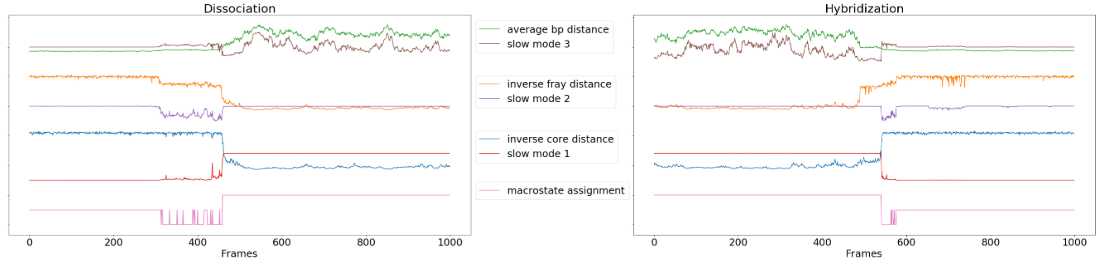
\includegraphics[width=120mm]{Figs/figs_imp/GC-core_tracking_modes.png}
        \caption{Leading GC-core SRV coordinates correlated with identifiable physical coordinates during sample hybridization (a) and dissociation (b) events. (c) Pearson correlations between all 100 intermolecular base pair distances and each the three leading slow modes. SRV2 correlations were calculated in the H and F4 states; SRV correlations were calculated in the D state.}
        \label{fig:GC-core_tracking_modes}
	\end{center}
\end{figure}    

% not sure if this should directly follow the SRV-MSM GC-core description or directly follow the GC-core dmaps?
% try cutting this out entirely ?
%\subsection{SRV correlations to physical coordinates}

Having constructed and interpreted SRV-MSMs, we revisited our original SRV basis to investigate how slow modes are constructed from input features. We found these GC-core modes to be of particular interest as they reveal the hierarchical and nonlinear nature of the dynamical encoding. We examined a collection of "trimmed" trajectories centered on both hybridization or dissociation events. For each trajectory, we compared the first three SRV coordinates with a corresponding collective variables with which they shared behavior. Two representative trajectories are shown in figure (\ref{fig:GC-core_tracking_modes}). Complementary G:C pairs are the best indicators for a hybridization/dissociation event, and we see a sharp change in the first SRV mode (SRV1) as these bonds form or break. The second slow mode (SRV2) is most active when G:C pairs are bound but the adjacent AT pairs are not. There is a small signal for fraying at the outer base pairs, but the mode overwhelmingly learns about these neighboring A:T/G:C bonds. Moreover, this behavior reflects movement in and out of the F4 state in the corresponding SRV-MSM discussed above. SRV3 is most active during dissociation, and seems to track closely with the average distance between all complementary base pairs. We attribute this to the SRV learning about the diffusive motions of the two body system and evaluating the likelihood of an imminent hybridization event. The third mode also peaks when the oligos are close together but configured in such a way that is not amenable hybridization. These misaligned conformations include inverse contacts where 5'/5' and 3'/3' ends meet and looped conformations where one strand is folded in on itself and preventing satisfactory WC contacts. 

Despite the qualitative trends we observe between physical coordinates and leading SRV modes, we found it difficult to find correlations across full trajectories. With the exception of SRV1, Pearson correlations between physical coordinates and SRV modes were near zero and showed erroneous trends. However, when we performed this analysis along smaller sections of trajectories we noticed that the sign of SRV2 and SRV3 correlations switched depending on whether the oligos were in the hybridized or dissociated state. This shows that these modes are inherently nonlinear and provide support on top of the first mode -- which serves as an indicator function for hybridized vs. dissociated state. With respect to our SRV-MSM macroscates, we found that SRV2 was "turned on" in the H and F4 states -- corresponding to the intact helix and frayed state, respectively -- and SRV3 was turned on in the dissociated state. Accordingly, we calculated Pearson correlations between each SRV mode and all distances in states where the modes are active. Figure \label{fig:GC-core_tracking_modes} shows the highest correlation between SRV2 and inner A:T pairs, weak correlation with outer A:T pairs, and an inverse correlation with 5'/5' and 3'/3' pairs which tend to approach each when the duplex is in the F4 state. We also observed a highly symmetric correlation between SRV3 and central base pairs distances, which indicative of overall diffusive behavior. Taken together, these analyses reveal how the SRV learns and represents the dynamical space in an hierarchical manner, providing enhanced resolution to a linear method like tICA and producing the MSM results we observe above.

\subsection{Structural diversity in the F4 state informs fraying dynamics} 

\begin{figure}[ht!]
	\begin{center}
        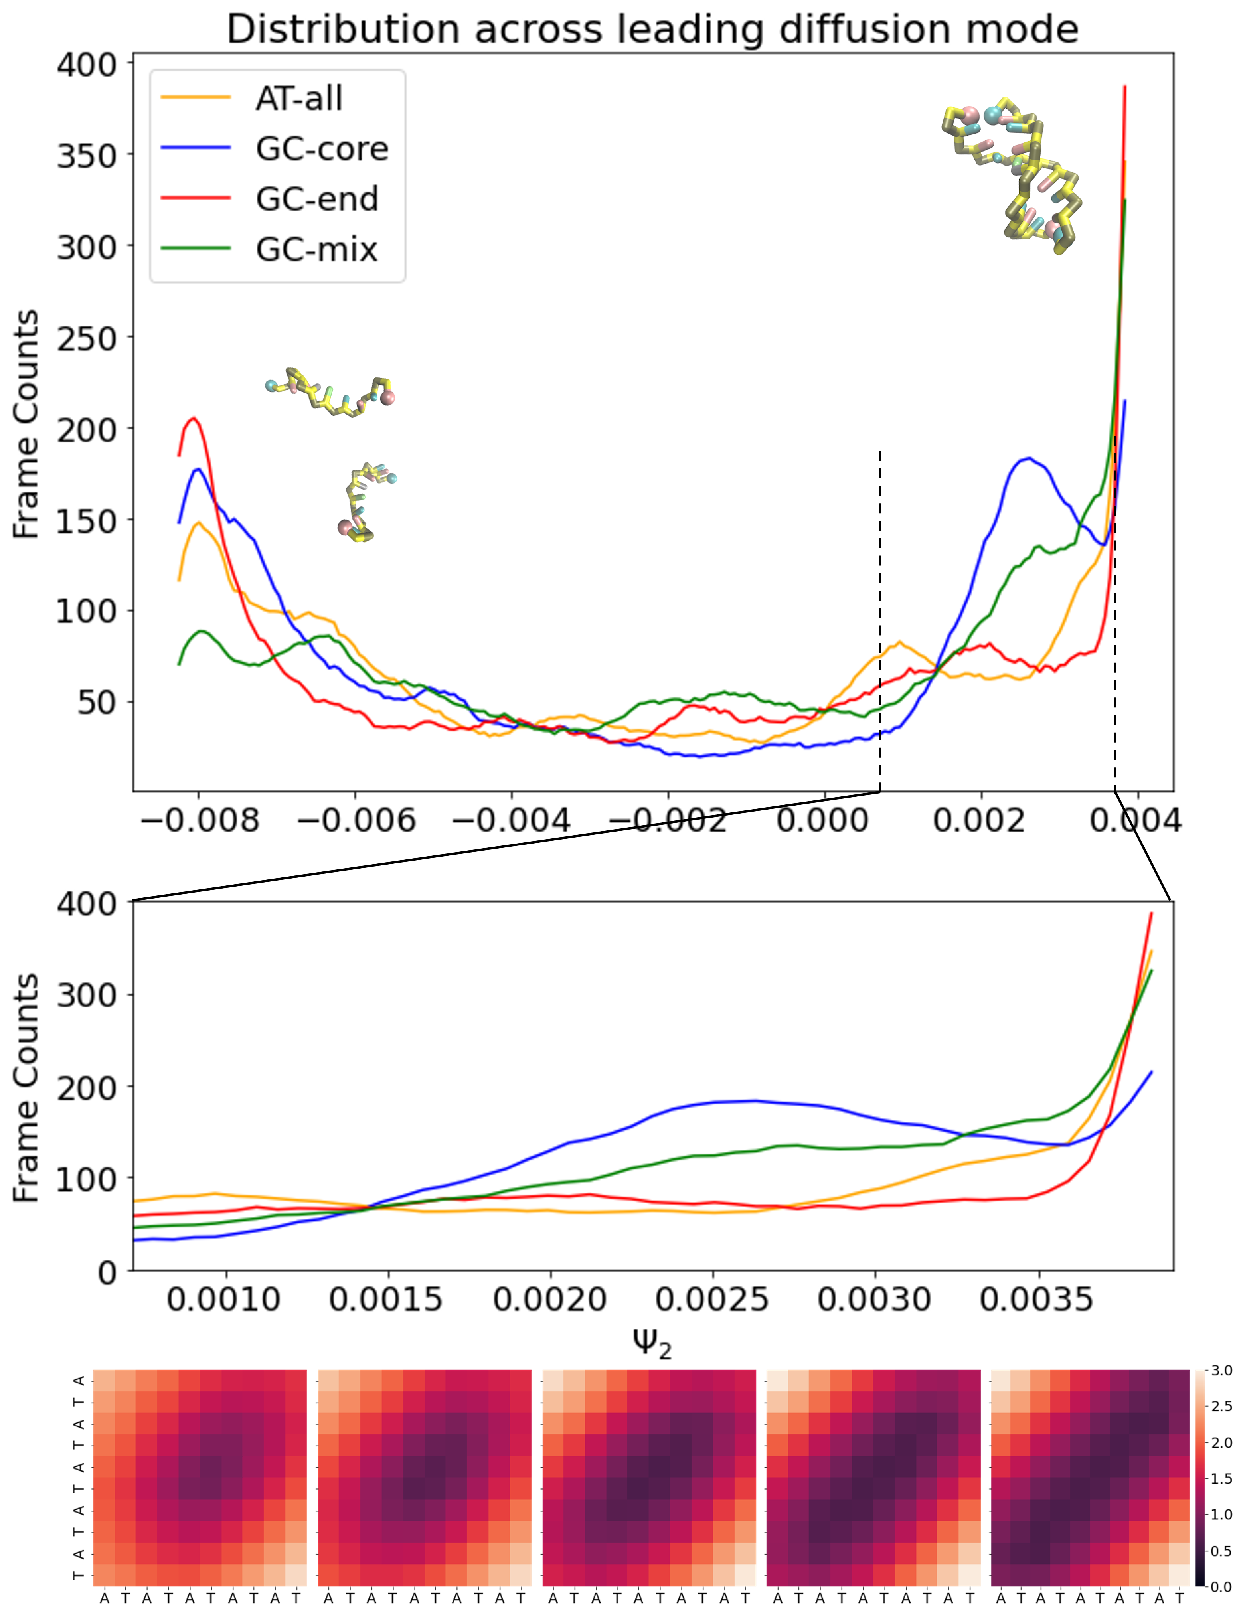
\includegraphics[width=450, scale=1]{Fig9.pdf}
        \caption{Diffusion map representation configurations sampled from the F4 state. The x and y axes represent the the first two non-trivial diffusion map eigenfunctions. Color maps show the probability that conformations are clustered into the frayed macrostate, maximum distance between 4th AT basepairs, and the overlap between adjacent A:T basepairs and the GC core.}
        \label{fig:GC-core_dmaps}
	\end{center}
\end{figure}

% shift to include this in the overall diffusion map section
%\subsubsection{Diffusion maps show ensemble of frayed states}

We applied a similar diffusion map approach to investigate the structural composition of the F4 macrostate. We build diffusion maps using 10000 frames sampled from the macrostate (figure \ref{fig:GC-core_dmaps}). Again, we were able to identify a combination of physical coordinates that closely correlated to the first two non-trivial diffusion modes. We found that a larger distance between internal A:T pairs increased the PCCA+ probability of inclusion into macrostate. This distance also correlated closely with the second diffusion map mode. Interestingly, we observed that the first non-trivial mode -- the feature that describes the most structural diversity in the system -- corresponds to difference in "overlap" distance between adjacent A or T bases and the GC core. We defined overlap as the distance between a G/C and the A/T adjacent to its native complement. At the extremes of this coordinate, one strand maintains most of its helical character while the other twists out of place. Because WC bonds are obstructed by the oligomer, the other strand is likely to fray before contacts can reform, or, less frequently, the duplex undergoes full dissociation. Interchange between these substates illustrate how the the F4 can maintain a longer lifetime compared to other A:T terminal sequences. 


\subsection{Explicit model comparisons}

We also acknowledge that the implicit model may not fully capture the role of ions in facilitating hybridization and dissociation. In addition to implicit simulations, we followed the same pipeline to generate simulations and SRV-MSMs given the ion conditions specified in the \citet{Sanstead2016} using the 3spn2 explicit implementation \citep{Hinckley2015}. These results look very similar to the implicit case, although with slightly slower dynamics and higher uncertainty in stationary probabilities. Comparisons were limited by the higher computational demand required to simulate 5x the beads in the box, a shorter integration timestep, and reliance on Ewald summation to account for electrostatics. We caution over-interpretation of these results as the explicit model has not been as widely adopted or thoroughly validated compared to the implicit model.


\begin{figure}[ht!]
	\begin{center}
        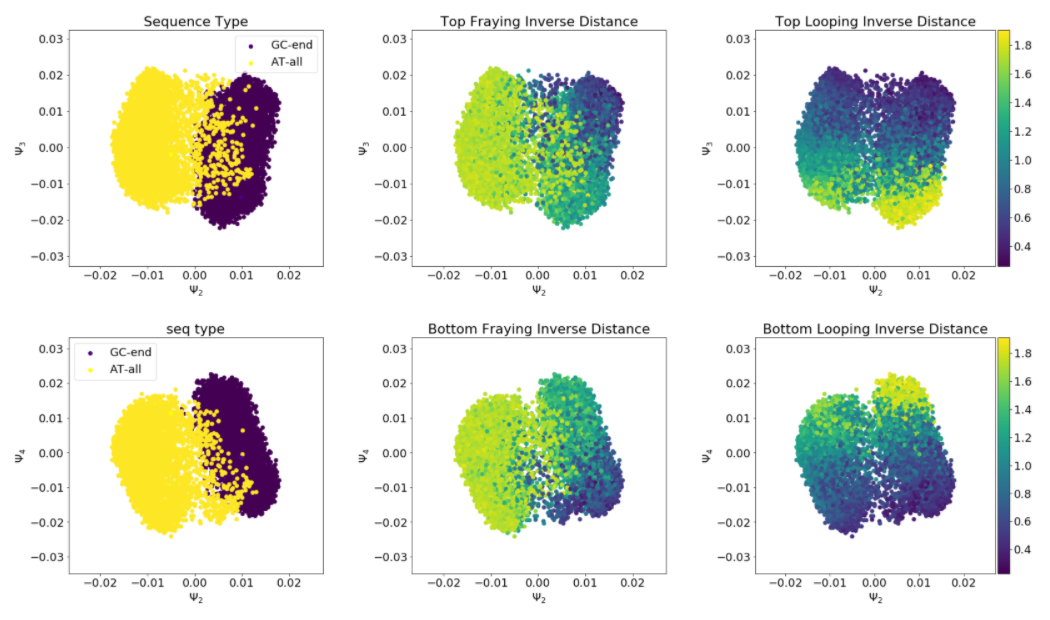
\includegraphics[width=\textwidth]{Figs/figs_imp/GC-end_dmaps_full.PNG}
        \caption{Full 5' diffusion maps including degenerate third diffusion map mode.}
        \label{fig:GC-end_dmaps_full}
	\end{center}
\end{figure}

\begin{figure}[ht!]
	\begin{center}
        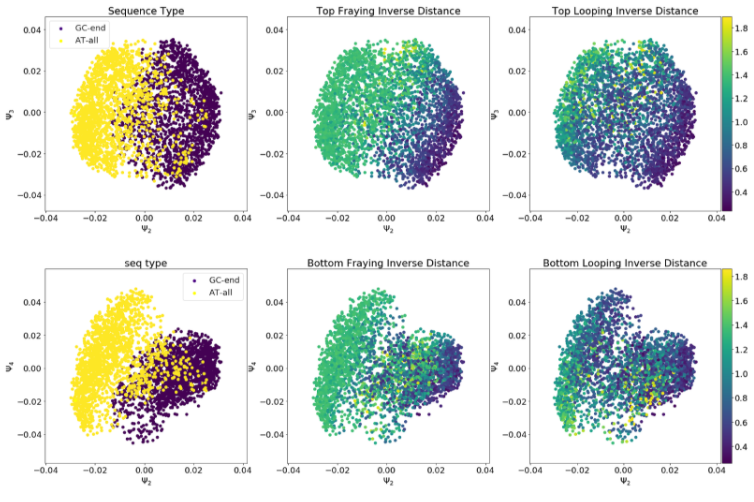
\includegraphics[width=\textwidth]{Figs/figs_imp/GC-end_dmaps_3prime.PNG}
        \caption{Full 3' diffusion maps, shows greater overlap between the AT-all and GC-end populations, as well as a less distinct "looping" region for intact GC bonds}
        \label{fig:GC-end_dmaps_3prime}
	\end{center}
\end{figure}

% add figure for slow and fast response fitting (just GC-core)
\begin{figure}[ht!]
	\begin{center}
        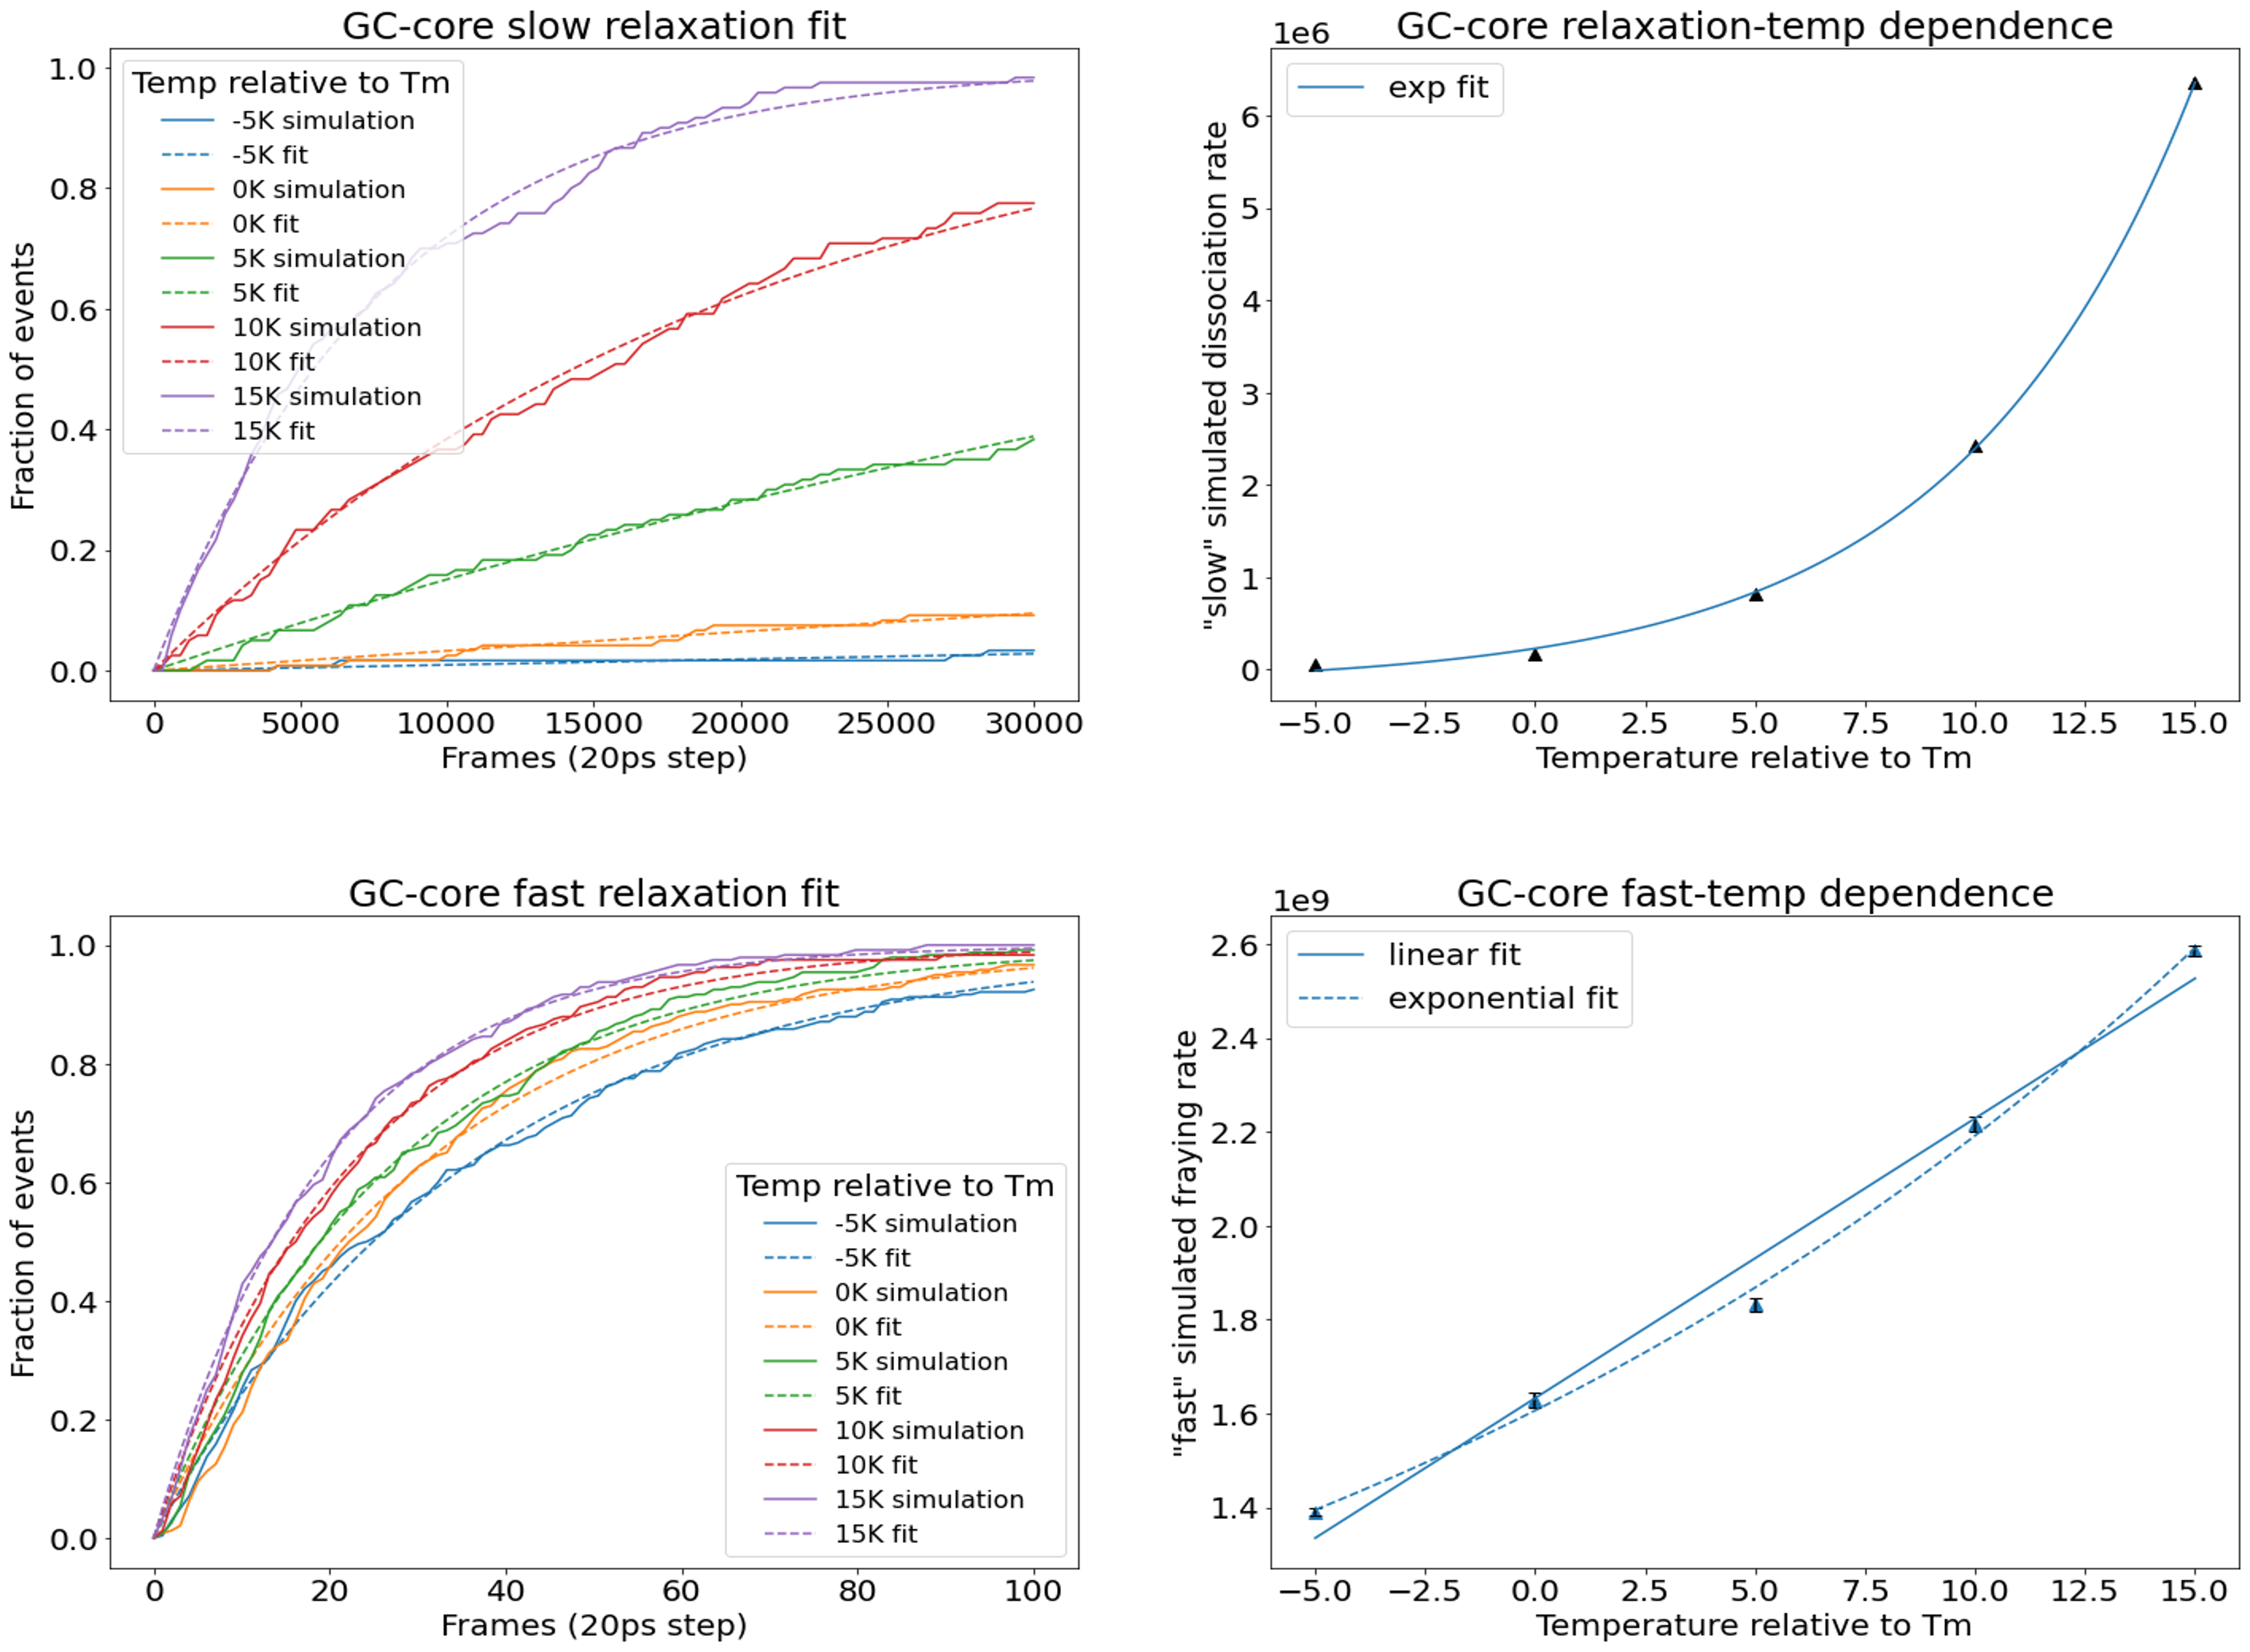
\includegraphics[width=\textwidth]{Figs/figs_imp/Tjump_fast_slow_fits.png}
        \caption{Slow and Fast modes were determined by fitting over a distribution of 120 independent simulations. For each temperature in the series, a relaxation curve was fit to the distribution and the associated exponential coefficient was used to the calculate rate. Temperatures series between -5 - +15K relative to empirically determined sequence melting temperature were explored. This process was repeated for each sequence (only GC-core is shown above).}
        \label{fig:fast_slow_fits}
	\end{center}
\end{figure}


%add anymore figures for the time analysis: As shown bleow:
\begin{comment}


\subsubsection{\label{sec:Results}Code to provide on GitHub} 
\begin{enumerate}
    \item Cross val data
    \item lammps run script and each sequence input files
    \item Featurization with mdtraj (reindexing and sparse saving)
    \item Dmaps for GC-core and GC-end
    \item timescales comparison
    \item SRV cross valss
    \item MSM construction
    
\end{enumerate}
\end{comment}

\begin{comment}

\section{\label{sec:Discussion}Discussion}

\citep{Galindo-Murillo2015ConvergenceDGCACGAACGAACGAACGC}
Long simulations shows that terminal fraying does not converge on the picosecond timescale

\citep{Nonin1995TerminalFraying}
Most simulations suppress fraying by placing GC pairs at termini.

\citep{Andreatta2006UltrafastHelix}
- Base opening process is slower than 40 ns but faster than 1ms
- Open termini state shows new fraying mode of 5ps (I think shows free base motions)
\end{comment}

\begin{comment}

%%%%%% Other MSM and timescales approaches  %%%%%%%%%%%

McGibbon, R. T., & Pande, V. S. (2015). Variational cross-validation of slow dynamical modes in molecular kinetics : Importance of not generating too many microstates and employting cross-validation to avoid artificially high scores or artificially slow dynamics. Both of these lead to models fitting statistical noise which is the root of boosted scores.

Pinamonti, G., Paul, F., Rodriguez, A., & Bussi, G. (n.d.). analyzed with core-set Markov state models, 43: Good ideas on core-based clustering. Assigning microstates based on physical characteristics is interesting but didn't seem to work for me in practice (could try doing this based on sim.log data with number of base pairs bound or some energy metric). Lot's of notes on this paper regarding comparisons to timescales. Good notes on higher resolution fraying interactions that we likely can't resolve.

Sua, E., Adelman, J. L., & Zuckerman, D. M. (2016). Accurate Estimation of Protein Folding and Unfolding Times : Beyond Markov State Models, 1. https://doi.org/10.1021/acs.jctc.6b00339:
More accurate ways to adapt MFPT into a rate

Refs for DNA fraying:
\citep{Hagan2003AtomisticDNA} Atomistic simulations for biosensign app (can include in intro). Use TPS to focus on kinetic pathway by which singl base pair bind/unbind. Focus on end base of 3-bp oligomer in explicit solvent. Finds order parameters tracking base pair binding as well as intra-strand stacking. (energy and distance for each). 

\citep{Wong2008TheSimulations} Three step melting process: untwisting most important,

6K.-Y. Wong and B. M. Pettitt, “The pathway of oligomeric DNA melting investigated by molecular dynamics simulations,” Biophys. J. 95, 5618– 5626 (2008).
37A. Perez and M. Orozco, “Real-time atomistic description of DNA unfold- ing,” Angew. Chem. 49, 4805–4808 (2010).
38M. F. Hagan, A. R. Dinner, D. Chandler, and A. K. Chakraborty, “Atomistic understanding of kinetic pathways for single base-pair binding and unbinding

\end{comment}


\clearpage
\newpage

\bibliography{references}
%\bibliography{refs_mendeley2}

%%%%%%%%%%%%%%%%%%%%%%%%%%%%%%%%%%%%%%%%%%%%%%%%%%%%%%%%%%%%%%%%%%%%%
%% The "tocentry" environment can be used to create an entry for the
%% graphical table of contents.
%%%%%%%%%%%%%%%%%%%%%%%%%%%%%%%%%%%%%%%%%%%%%%%%%%%%%%%%%%%%%%%%%%%%%

\clearpage


\end{document}
